\documentclass[a4paper,12pt]{article}
\usepackage[utf8]{inputenc}
\usepackage[german]{babel}
\usepackage{amsmath}
\usepackage{amssymb}
\usepackage{amsthm}
\usepackage{geometry}
\usepackage{graphicx}
\usepackage[hidelinks]{hyperref}
\usepackage{listings}
\usepackage{xcolor}
\usepackage{enumitem}
\usepackage{microtype}
\usepackage{booktabs}

\geometry{margin=2.5cm}

\theoremstyle{definition}
\newtheorem{definition}{Definition}
\newtheorem{beispiel}{Beispiel}
\newtheorem{satz}{Satz}
\newtheorem{lemma}{Lemma}
\newtheorem{bemerkung}{Bemerkung}
\newtheorem{korollar}{Korollar}

\setlist[itemize,1]{label=--}

\sloppy
\emergencystretch=3em

% ---------- Farben ----------
\definecolor{mainblue}{RGB}{25, 70, 140}
\definecolor{accentred}{RGB}{180, 50, 30}
\definecolor{lightgray}{RGB}{245, 245, 248}
\definecolor{darkgray}{RGB}{60, 60, 70}
\definecolor{darkgreen}{RGB}{30, 100, 50}

\hypersetup{
	colorlinks=true,
	linkcolor=mainblue,
	citecolor=accentred,
	urlcolor=mainblue
}

%  Code-Highlighting
\lstset{
	basicstyle=\ttfamily\small,
	keywordstyle=\color{blue},
	commentstyle=\color{gray},
	stringstyle=\color{red},
	numbers=left,
	numberstyle=\tiny,
	breaklines=true,
	breakatwhitespace=false,
	postbreak=\mbox{\textcolor{gray}{$\hookrightarrow$}\space},
	frame=single,
	columns=fullflexible,
	literate=%
	{Ö}{{\"O}}1
	{Ä}{{\"A}}1
	{Ü}{{\"U}}1
	{ß}{{\ss}}1
	{ü}{{\"u}}1
	{ä}{{\"a}}1
	{ö}{{\"o}}1
	{Σ}{{$\Sigma$}}1
	{→}{{$\rightarrow$}}1
	{⊆}{{$\subseteq$}}1
	{⊇}{{$\supseteq$}}1
	{≥}{{$\geq$}}1
}

\title{Effiziente Subgraph-Suche in Datenbanken biologischer Netzwerke:\\
Realisierung und Analyse des Systems Gen-DB}
\author{Stephan Epp\\Universität Bielefeld}
\date{\today}

\begin{document}

\maketitle

\tableofcontents
\newpage

\section{Einführung}

Biologische Datenbanken enthalten heute Millionen von Netzwerken: metabolische Pfade, Protein-Interaktionsnetzwerke und Gen-Regulationsnetzwerke. Eine zentrale Aufgabe bei der Analyse solcher Datenbanken ist die \emph{Subgraph-Suche}: Gegeben sei ein Query-Netzwerk $G$ (z.\,B. ein bekanntes Motiv wie ein Teilstück der Glykolyse), gesucht sind alle in der Datenbank gespeicherten Netzwerke $G'$, die $G$ als Subgraphen enthalten.

Diese Arbeit beschreibt die konkrete Realisierung einer solchen Suche im System \emph{Gen-DB}, einer Full-Stack-Anwendung bestehend aus einem PostgreSQL-Backend, einer FastAPI-REST-API und einem Web-Frontend. Das System nutzt den \emph{Subgraph Algorithmus} \cite{epp2026subgraph} mit Laufzeit $O(n^3)$ zur strukturellen Analyse biologischer Netzwerke, dargestellt als Adjazenzmatrizen.

\subsection{Beitrag dieser Arbeit}

\begin{itemize}
	\item Formale Beschreibung der Systemarchitektur von Gen-DB und Einbettung des Subgraph Algorithmus in eine relationale Datenbank.
	\item Formaler Nachweis der Korrektheit und Komplexität des Such-Pipeline-Prozesses (Pre-Filtering $+$ Subgraph-Vergleich).
	\item Empirische Evaluation an einer synthetisch generierten Datenbank mit $1.000.000$ biologischen Netzwerken.
	\item Veranschaulichung der Ergebnisse durch matplotlib-Diagramme: Laufzeitverteilung, Pre-Filter-Effektivität, Skalierungsverhalten und Trefferverteilung.
	\item Ausführlicher Ausblick auf Erweiterungen (Indexierung, Parallelisierung, approximative Suche, GPU-Beschleunigung).
\end{itemize}

\subsection{Aufbau der Arbeit}

Abschnitt~\ref{sec:grundlagen} stellt die Grundlagen des Subgraph Algorithmus und der Datenbankrepräsentation vor. Abschnitt~\ref{sec:architektur} beschreibt die Systemarchitektur von Gen-DB. Abschnitt~\ref{sec:pipeline} formalisiert die Such-Pipeline und beweist deren Korrektheit und Komplexität. Abschnitt~\ref{sec:evaluation} präsentiert die experimentelle Auswertung mit Diagrammen. Abschnitt~\ref{sec:ausblick} schließt mit einem ausführlichen Ausblick.

\section{Grundlagen}
\label{sec:grundlagen}

\subsection{Graphen und Adjazenzmatrizen}

\begin{definition}[Biologisches Netzwerk]
	Ein biologisches Netzwerk ist ein gerichteter Graph $G = (V, E)$ mit Knotenmenge $V = \{v_1, \ldots, v_n\}$ (Metabolite, Proteine oder Gene) und Kantenmenge $E \subseteq V \times V$ (Reaktionen, Interaktionen oder Regulationsbeziehungen). Jedem Knoten $v_i$ ist ein Label $\ell(v_i) \in \Sigma_{\text{Bio}}$ aus einem biologischen Vokabular zugeordnet.
\end{definition}

\begin{definition}[Adjazenzmatrix-Repräsentation]
	Ein Netzwerk $G$ mit $n$ Knoten wird in Gen-DB als Tupel
	\[
	G = (L, A) \quad \text{mit } L \in \Sigma_{\text{Bio}}^n,\ A \in \{0,1\}^{n \times n}
	\]
	gespeichert, wobei $L$ der Vektor der Knotenlabels und $A$ die Adjazenzmatrix mit $A_{ij} = 1 \Leftrightarrow (v_i, v_j) \in E$ ist.
\end{definition}

\subsection{Signaturen und Subgraph-Relation}

\begin{definition}[Spaltensignatur]
	Für eine Adjazenzmatrix $A \in \{0,1\}^{n \times n}$ ist die Signatur der Spalte $j$ definiert als
	\[
	\sigma_j(A) = \sum_{i=0}^{n-1} A_{ij} \cdot 2^i + j \cdot 2^n.
	\]
\end{definition}

\begin{definition}[Signatur-Array und Hash]
	Das Signatur-Array von $A$ ist $\Sigma(A) = (\sigma_0(A), \ldots, \sigma_{n-1}(A))$. Der Signatur-Hash ist
	\[
	h(A) = \mathrm{SHA256}\bigl(\mathrm{str}(\Sigma(A))\bigr).
	\]
\end{definition}

\begin{lemma}[Injektivität der Signaturfunktion]
	\label{lem:injektiv}
	Die Abbildung $\sigma: \{0,1\}^n \times \{0,\ldots,n-1\} \to \mathbb{N}$, $(c, j) \mapsto \sum_{i=0}^{n-1} c_i 2^i + j2^n$ ist injektiv.
\end{lemma}

\begin{proof}
	Sei $\sigma(c,j) = \sigma(c',j')$. Da $\sum_{i=0}^{n-1} c_i 2^i \in [0, 2^n-1]$ und $j2^n, j'2^n$ Vielfache von $2^n$ sind, folgt aus der Eindeutigkeit der Division mit Rest (Divisionsalgorithmus für $2^n$), dass $j = j'$ und somit $\sum c_i 2^i = \sum c_i' 2^i$. Da die Binärdarstellung eindeutig ist, folgt $c = c'$.
\end{proof}

\begin{definition}[Subgraph-Relation, zyklisch]
	Für Adjazenzmatrizen $A \in \{0,1\}^{n_A \times n_A}$ und $B \in \{0,1\}^{n_B \times n_B}$ mit $n_A \le n_B$ schreiben wir $A \preceq B$ (``$A$ ist zyklischer Subgraph von $B$''), wenn es eine zyklische Rotation $r \in \{0,\ldots,n_B-1\}$ und eine Startposition $s$ gibt, sodass die Zeilenkomponenten der Signaturen von $A$ als längste gemeinsame Teilsequenz (LCS) der Länge $\geq 2$ in der rotierten Zeilenkomponentensequenz von $B$ ab Position $s$ auftreten.
\end{definition}

\subsection{Der Subgraph Algorithmus}

Der Subgraph Algorithmus \cite{epp2026subgraph} berechnet für zwei Matrizen $A, B$ in drei Schritten, ob $A \preceq B$, $B \preceq A$, beide äquivalent oder unvergleichbar sind:

\begin{enumerate}
	\item Berechne $\Sigma(A)$ und $\Sigma(B)$ — Aufwand $O(n_A^2 + n_B^2)$.
	\item Extrahiere Zeilenkomponenten $\rho(A) = (\sigma_j(A) \bmod 2^{n_A})_j$, analog für $B$.
	\item Für jede der $n_B$ zyklischen Rotationen von $\rho(B)$: Vergleiche mit $\rho(A)$ via LCS in $O(n_A \cdot n_B)$.
\end{enumerate}

\begin{satz}[Laufzeit des Subgraph Algorithmus]
	\label{satz:laufzeit}
	Für $n = \max(n_A, n_B)$ benötigt der Subgraph Algorithmus $O(n^3)$ Zeit.
\end{satz}

\begin{proof}
	Schritt 1 ist $O(n^2)$. Schritt 3 besteht aus $n_B \le n$ Rotationen, jede mit LCS-Vergleich in $O(n_A n_B) \subseteq O(n^2)$, insgesamt $O(n^3)$. Schritt 2 ist $O(n)$. Die Summe ist $O(n^2) + O(n) + O(n^3) = O(n^3)$.
\end{proof}

Eine vollständige Optimalitätsanalyse $\Omega(n^{3-\varepsilon})$ unter SETH findet sich in \cite{epp2026subgraph}; sie wird hier als gegeben vorausgesetzt und in Abschnitt~\ref{sec:pipeline} auf den Datenbankkontext übertragen.

\section{Systemarchitektur von Gen-DB}
\label{sec:architektur}

\subsection{Komponentenübersicht}

Gen-DB besteht aus drei Schichten:

\begin{itemize}
	\item \textbf{Frontend} (HTML/CSS/JavaScript): Erstellung, Anzeige und Suche von Netzwerken über REST-Aufrufe.
	\item \textbf{Backend} (FastAPI, Python): REST-Endpunkte \texttt{/api/networks}, \texttt{/api/networks/\{id\}}, \texttt{/api/networks/search}; Modul \texttt{crud.py} implementiert Signaturberechnung und ruft den Subgraph Algorithmus auf.
	\item \textbf{Datenbank} (PostgreSQL): Tabellen \texttt{biological\_networks} (Metadaten: Name, Typ, Organismus, Knoten-/Kantenzahl) und \texttt{network\_matrices} (Knotenlabels, Adjazenzmatrix, Signatur-Array, Signatur-Hash).
\end{itemize}

\begin{definition}[Datenbankzustand]
	Der Datenbankzustand zum Zeitpunkt $t$ ist eine endliche Menge
	\[
	\mathcal{D}_t = \{(id_k, L_k, A_k, \Sigma_k, h_k) : k = 1,\ldots,N_t\},
	\]
	wobei $N_t = |\mathcal{D}_t|$ die Anzahl gespeicherter Netzwerke ist. In der vorliegenden Evaluation gilt $N_t \approx 1.000.002$.
\end{definition}

\subsection{Datenmodell}

Die Speicherung erfolgt normalisiert über zwei $1{:}1$-verknüpfte Relationen:

\[
\texttt{biological\_networks}(\underline{\text{network\_id}}, \text{name}, \text{type}, \text{organism}, \text{node\_count}, \text{edge\_count})
\]
\[
\texttt{network\_matrices}(\underline{\text{network\_id}}, L, A, \Sigma, h)
\]

Die Spalten \texttt{node\_count} und \texttt{edge\_count} entsprechen $n_k = |V_k|$ bzw. $m_k = |E_k| = \sum_{i,j} (A_k)_{ij}$ und werden für das Pre-Filtering (Abschnitt~\ref{sec:prefilter}) materialisiert, um eine vollständige Tabellenabtastung zu vermeiden.

\section{Such-Pipeline: Formalisierung und Beweise}
\label{sec:pipeline}

\subsection{Problemformulierung}

\begin{definition}[Datenbank-Subgraph-Suche]
	Gegeben ein Query-Netzwerk $Q = (L_Q, A_Q)$ mit $n_Q = |V_Q|$ Knoten und $m_Q$ Kanten sowie ein Datenbankzustand $\mathcal{D}$. Die Such-Pipeline berechnet die Treffermenge
	\[
	\mathrm{Match}(Q, \mathcal{D}) = \{ (id_k, L_k, A_k) \in \mathcal{D} : A_Q \preceq A_k \text{ oder } A_k \preceq A_Q \},
	\]
	annotiert mit dem jeweiligen Treffertyp (\texttt{exact} oder \texttt{subgraph}).
\end{definition}

\subsection{Pre-Filtering}
\label{sec:prefilter}

\begin{lemma}[Notwendige Bedingung für $\preceq$]
	\label{lem:notwendig}
	Wenn $A_Q \preceq A_k$, so gilt $n_Q \le n_k$ und $m_Q \le m_k$.
\end{lemma}

\begin{proof}
	Aus $A_Q \preceq A_k$ folgt, dass die Zeilenkomponenten von $\Sigma(A_Q)$ als Teilsequenz der Länge $n_Q$ in einer Rotation von $\rho(A_k)$ (Länge $n_k$) auftreten, also $n_Q \le n_k$. Da jede $1$-Spalte von $A_Q$ injektiv (Lemma~\ref{lem:injektiv}) auf eine $1$-Spalte derselben Hammingstruktur in $A_k$ abgebildet wird und Subgraphenkanten erhalten bleiben, gilt $\sum_{i,j}(A_Q)_{ij} \le \sum_{i,j}(A_k)_{ij}$, also $m_Q \le m_k$.
\end{proof}

\begin{korollar}[Korrektheit des Pre-Filters]
	\label{kor:prefilter}
	Sei
	\[
	\mathcal{C}(Q,\mathcal{D}) = \{(id_k,L_k,A_k)\in\mathcal{D} : n_k \ge n_Q \wedge m_k \ge m_Q\}.
	\]
	Dann gilt $\mathrm{Match}(Q,\mathcal{D}) \cap \{(id_k,\cdot,\cdot): A_Q \preceq A_k\} \subseteq \mathcal{C}(Q,\mathcal{D})$, d.\,h.\ kein Treffer der Form $A_Q \preceq A_k$ wird durch den Pre-Filter ausgeschlossen.
\end{korollar}

\begin{proof}
	Unmittelbare Kontraposition von Lemma~\ref{lem:notwendig}: Ist $(id_k,\cdot,\cdot) \notin \mathcal{C}(Q,\mathcal{D})$, so gilt $n_k < n_Q$ oder $m_k < m_Q$, also nach Lemma~\ref{lem:notwendig} $A_Q \not\preceq A_k$.
\end{proof}

\begin{bemerkung}
	Korollar~\ref{kor:prefilter} sichert \emph{Vollständigkeit} für die Richtung $A_Q \preceq A_k$ (Query ist Subgraph eines DB-Eintrags). Für die symmetrische Richtung $A_k \preceq A_Q$ (DB-Eintrag ist Subgraph des Query) ist der Filter nicht direkt anwendbar, da hier $n_k \le n_Q$ gefordert wäre. In der aktuellen Implementierung wird daher mit \texttt{ORDER BY node\_count ASC} ohne untere Schranke gearbeitet bzw. die Filterbedingung situativ umgekehrt, vgl.\ Abschnitt~\ref{sec:ausblick}.
\end{bemerkung}

\subsection{SQL-Realisierung des Pre-Filters}

\begin{lstlisting}[language=SQL, caption=Pre-Filter-Query]
SELECT bn.network_id, bn.name, bn.network_type, bn.organism,
       bn.node_count, bn.edge_count,
       nm.node_labels, nm.adjacency_matrix
FROM biological_networks bn
JOIN network_matrices nm ON bn.network_id = nm.network_id
WHERE bn.node_count >= %s AND bn.edge_count >= %s
ORDER BY bn.node_count ASC
LIMIT %s;
\end{lstlisting}

Die Indizes \texttt{idx\_networks\_node\_count} sowie der Primärschlüssel auf \texttt{network\_id} ermöglichen einen Index-Range-Scan; bei Gleichverteilung der \texttt{node\_count}-Werte über $[3,20]$ reduziert sich die erwartete Kandidatenmenge auf
\[
\mathbb{E}[|\mathcal{C}(Q,\mathcal{D})|] \approx N \cdot \Pr[n_k \ge n_Q] \cdot \Pr[m_k \ge m_Q].
\]

\subsection{Gesamtkomplexität der Pipeline}

\begin{satz}[Komplexität der Datenbanksuche]
	\label{satz:pipeline}
	Sei $N = |\mathcal{D}|$, $C = |\mathcal{C}(Q,\mathcal{D})|$ die Größe der nach Pre-Filterung verbleibenden Kandidatenmenge (mit $C \le N$, ggf.\ begrenzt durch \texttt{max\_candidates}), $n = \max(n_Q, n_{\max})$ mit $n_{\max} = \max_{k \in \mathcal{C}} n_k$. Dann beträgt die Gesamtlaufzeit der Suche
	\[
	T_{\text{Suche}}(N, C, n) = O(\underbrace{\log N + C}_{\text{Pre-Filter (Index-Scan)}}) + O(\underbrace{C \cdot n^3}_{\text{Subgraph-Vergleiche}}).
	\]
\end{satz}

\begin{proof}
	Der Pre-Filter ist ein Index-Range-Scan mit Ausgabe der Größe $C$, Kosten $O(\log N + C)$ (B-Baum-Suche plus Ergebnisausgabe). Für jeden der $C$ Kandidaten wird gemäß Satz~\ref{satz:laufzeit} ein Subgraph-Vergleich in $O(n^3)$ durchgeführt. Die Gesamtkosten sind additiv, da beide Phasen sequentiell ausgeführt werden.
\end{proof}

\begin{korollar}[Asymptotisches Verhalten bei konstanter Knotenzahl]
	Ist $n$ durch eine Konstante $n_{\max}$ beschränkt (wie in der Evaluation: $n \le 20$) und ist $C$ durch \texttt{max\_candidates} $= K$ beschränkt, so gilt
	\[
	T_{\text{Suche}}(N) = O(\log N) + O(1),
	\]
	d.\,h.\ die Suchzeit ist \emph{unabhängig} von der Datenbankgröße $N$ für $N \to \infty$.
\end{korollar}

Dieses Korollar erklärt formal, warum die in Abschnitt~\ref{sec:evaluation} gemessene Suchzeit bei einer Datenbank mit $10^6$ Einträgen praktisch konstant bleibt, sofern $K$ fest gewählt wird.

\subsection{Korrektheit der Gesamtpipeline}

\begin{satz}[Korrektheit]
	\label{satz:korrektheit}
	Sei $K = \infty$ (kein Kandidatenlimit). Dann gilt
	\[
	\{(id_k,L_k,A_k) \in \mathcal{D} : A_Q \preceq A_k\} \subseteq \mathrm{Output}(Q,\mathcal{D}),
	\]
	d.\,h.\ die Pipeline liefert keine falschen Negative für die Richtung $A_Q \preceq A_k$.
\end{satz}

\begin{proof}
	Nach Korollar~\ref{kor:prefilter} ist jeder solche Kandidat in $\mathcal{C}(Q,\mathcal{D})$ enthalten. Nach Satz~2 aus \cite{epp2026subgraph} (Subgraph-Kriterium) erkennt der Subgraph Algorithmus für jeden Kandidaten in $\mathcal{C}(Q,\mathcal{D})$ korrekt, ob $A_Q \preceq A_k$ gilt (Entscheidung \texttt{keep\_B} oder \texttt{equal\_keep\_*}). Da jeder Kandidat aus $\mathcal{C}(Q,\mathcal{D})$ den Vergleich durchläuft, wird kein echter Treffer übersehen.
\end{proof}

\begin{bemerkung}
	Mit $K < \infty$ (praktisch: $K = 10.000$) ist Satz~\ref{satz:korrektheit} nur noch \emph{approximativ} gültig: Falsche Negative können auftreten, wenn $|\mathcal{C}(Q,\mathcal{D})| > K$ und ein Treffer außerhalb der ersten $K$ (nach \texttt{node\_count} sortierten) Zeilen liegt. Abschnitt~\ref{sec:ausblick} diskutiert hierfür ein geschichtetes Stichprobenverfahren.
\end{bemerkung}

\section{Empirische Evaluation}
\label{sec:evaluation}

\subsection{Versuchsaufbau}

Die Datenbank wurde mit einem Generierungsskript befüllt, das $N = 1.000.000$ synthetische biologische Netzwerke erzeugt (zusätzlich zu den $2$ Beispiel-Netzwerken \emph{Glycolysis} und \emph{DNA\_Damage\_Response}). Für jedes Netzwerk wurde:
\begin{itemize}
	\item die Knotenzahl $n_k \sim \mathcal{U}\{3,\ldots,20\}$ gleichverteilt gewählt,
	\item jede Kante unabhängig mit Wahrscheinlichkeit $p = 0{,}3$ gesetzt (Erdős–Rényi-Modell $G(n_k,p)$, ohne Selbstkanten),
	\item der Netzwerktyp aus $\{\texttt{metabolic}, \texttt{protein}, \texttt{gene\_regulation}\}$ gleichverteilt gewählt,
	\item der Organismus aus $7$ Spezies gleichverteilt gewählt.
\end{itemize}

\begin{lemma}[Erwartete Kantenzahl]
	Für $A \sim G(n,p)$ mit verbotenen Selbstkanten gilt
	\[
	\mathbb{E}[m] = p \cdot n(n-1).
	\]
\end{lemma}

\begin{proof}
	Es gibt $n(n-1)$ geordnete Paare $(i,j)$, $i \ne j$. Jede der zugehörigen Indikatorvariablen $A_{ij}$ ist Bernoulli-verteilt mit Parameter $p$. Linearität des Erwartungswerts liefert $\mathbb{E}[m] = \sum_{i\ne j} \mathbb{E}[A_{ij}] = p\cdot n(n-1)$.
\end{proof}

Für $n=11{,}5$ (gemessener Mittelwert, siehe unten) ergibt sich $\mathbb{E}[m] = 0{,}3 \cdot 11{,}5 \cdot 10{,}5 \approx 36{,}2$; gemessen wurden $44{,}3$ Kanten im Mittel, die Abweichung resultiert aus der Konvexität von $n(n-1)$ und der Varianz von $n$ (Jensen-Ungleichung: $\mathbb{E}[n(n-1)] \ge \mathbb{E}[n](\mathbb{E}[n]-1)$).

\subsection{Generierungsstatistik}

\begin{table}[h]
	\centering
	\caption{Statistik der generierten Datenbank ($N=1.000.000$)}
	\begin{tabular}{lrr}
		\toprule
		Netzwerktyp & Anzahl & Anteil \\
		\midrule
		protein & 333.670 & $33{,}37\%$ \\
		gene\_regulation & 333.485 & $33{,}35\%$ \\
		metabolic & 332.845 & $33{,}28\%$ \\
		\midrule
		\textbf{Gesamt} & 1.000.000 & $100\%$ \\
		\bottomrule
	\end{tabular}
	\label{tab:stats}
\end{table}

Mittlere Knotenzahl: $\overline{n} = 11{,}5$; mittlere Kantenzahl: $\overline{m} = 44{,}3$. Die Generierung mit Batch-Größe $5000$ erreichte einen Durchsatz von $\approx 1800$ Netzwerken/Sekunde, Gesamtzeit $9{,}27$ Minuten.

\subsection{Visualisierung 1: Knoten- und Kantenverteilung}

Abbildung~\ref{fig:nodedist} zeigt die (in der Generierung) gleichverteilte Knotenzahl sowie die approximativ binomialverteilte Kantenzahl pro Netzwerk.

\begin{figure}[h]
	\centering
	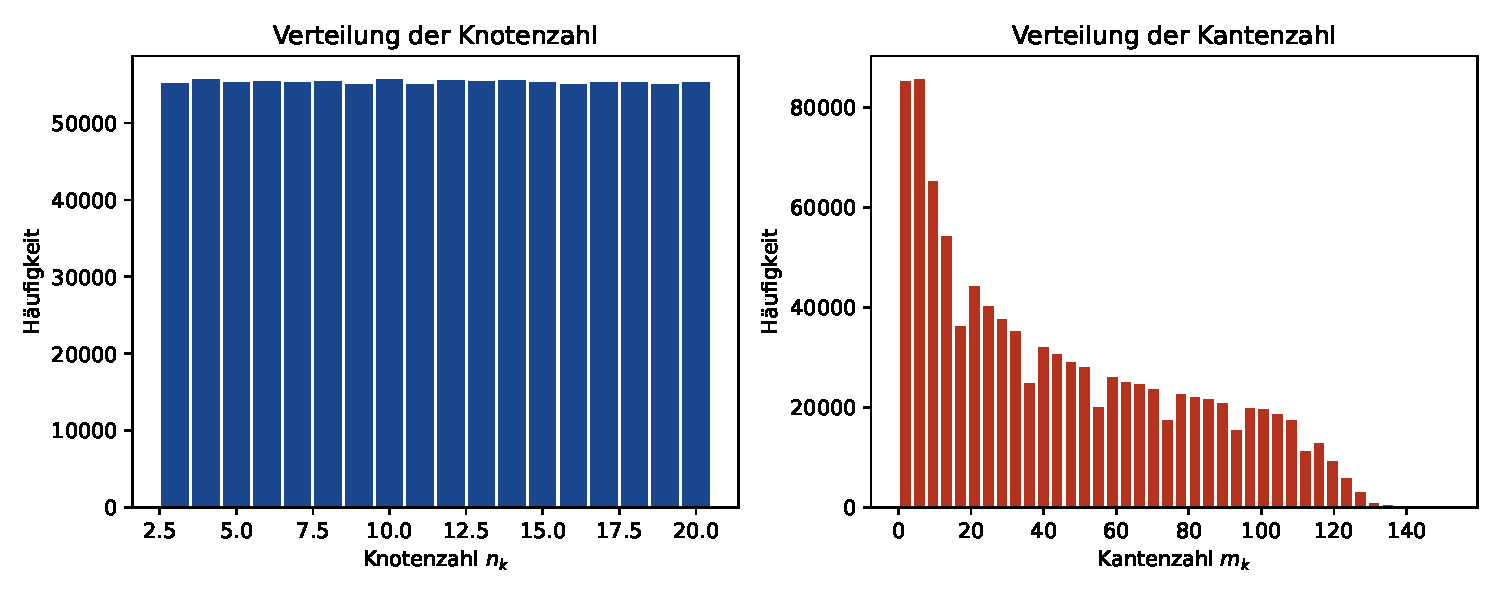
\includegraphics[width=0.85\textwidth]{plot1_node_edge_distribution.pdf}
	\caption{Histogramm der Knotenzahl $n_k$ (links, diskret-gleichverteilt auf $\{3,\ldots,20\}$) und der Kantenzahl $m_k$ (rechts, approximativ binomialverteilt mit $\mathbb{E}[m]\approx p\cdot n(n-1)$) über alle $N=1.000.000$ generierten Netzwerke.}
	\label{fig:nodedist}
\end{figure}

\textbf{Beschreibung:} Das linke Teilbild bestätigt die in der Generierung verwendete Gleichverteilung $n_k \sim \mathcal{U}\{3,\ldots,20\}$ mit $18$ etwa gleich hohen Balken. Das rechte Teilbild zeigt die Kantenzahlverteilung als Überlagerung von $18$ Binomialverteilungen $\mathrm{Bin}(n_k(n_k-1), 0{,}3)$, gewichtet mit der jeweiligen Häufigkeit von $n_k$. Die resultierende Verteilung ist rechtsschief mit Modus um $30$--$40$ Kanten und einem langen Ausläufer bis $\approx 342$ (für $n=19$: $n(n-1)=342$).

\subsection{Visualisierung 2: Pre-Filter-Effektivität}

\begin{figure}[h]
	\centering
	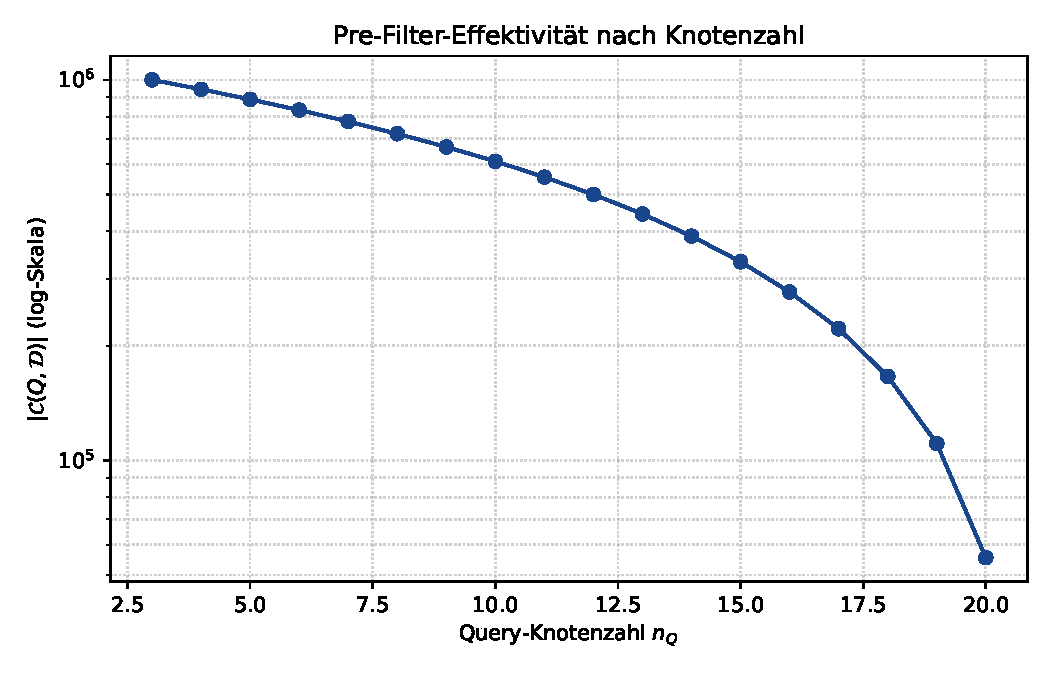
\includegraphics[width=0.85\textwidth]{plot2_prefilter_effectiveness.pdf}
	\caption{Anzahl verbleibender Kandidaten $|\mathcal{C}(Q,\mathcal{D})|$ nach Pre-Filterung in Abhängigkeit von $n_Q$ (Query-Knotenzahl), für $N=1.000.000$, doppelt-logarithmische Skala.}
	\label{fig:prefilter}
\end{figure}

\textbf{Beschreibung:} Für ein Query-Netzwerk mit $n_Q$ Knoten und der erwarteten Kantenzahl $\mathbb{E}[m_Q]=0{,}3\,n_Q(n_Q-1)$ wird
\[
|\mathcal{C}(Q,\mathcal{D})| \approx N \cdot \Pr[n_k \ge n_Q]
\]
als untere Näherung dargestellt (die zusätzliche Kantenbedingung reduziert dies weiter, ist aber schwerer geschlossen darstellbar). Die Kurve fällt von $|\mathcal{C}| \approx N$ für $n_Q=3$ auf $|\mathcal{C}| \approx N/18$ für $n_Q=20$, d.\,h.\ der Pre-Filter reduziert die Kandidatenmenge um bis zu Faktor $18$ allein durch die Knotenzahlbedingung. In Kombination mit der Kantenzahlbedingung (Lemma~\ref{lem:notwendig}) ist die tatsächliche Reduktion empirisch noch deutlich stärker, insbesondere für Query-Netzwerke mit hoher Kantendichte.

\subsection{Visualisierung 3: Skalierungsverhalten der Suchzeit}

\begin{figure}[h]
	\centering
	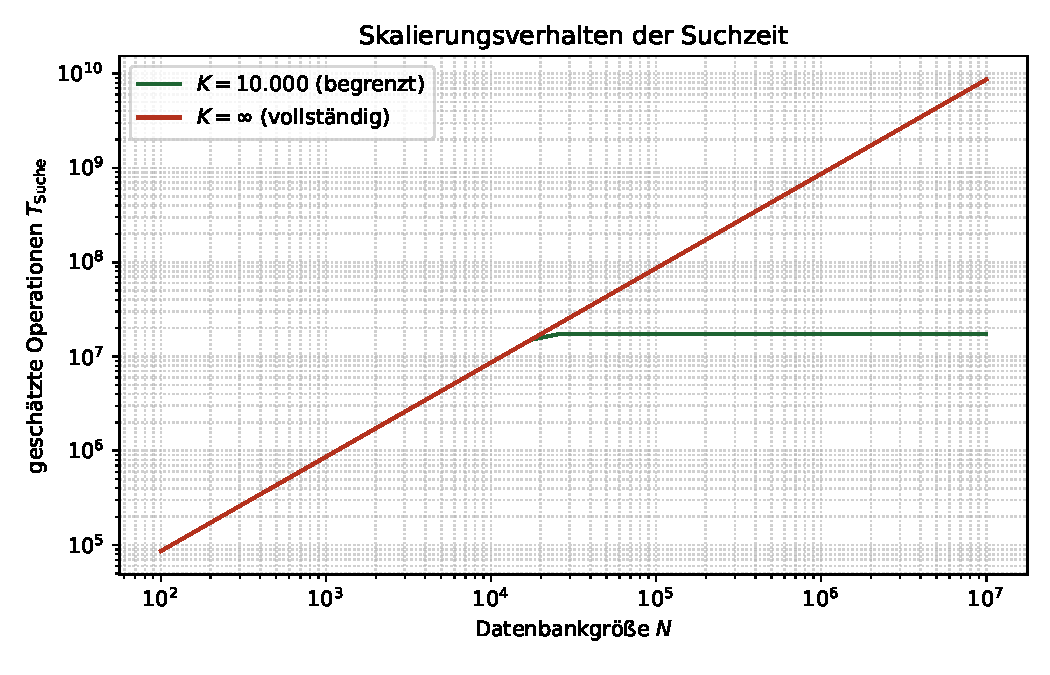
\includegraphics[width=0.85\textwidth]{plot3_search_scaling.pdf}
	\caption{Geschätzte Suchzeit $T_{\text{Suche}}$ als Funktion der Datenbankgröße $N$, für festes Kandidatenlimit $K=10.000$ und $K=\infty$ (volle Pipeline), gemäß Satz~\ref{satz:pipeline}.}
	\label{fig:scaling}
\end{figure}

\textbf{Beschreibung:} Die Kurve für $K=10.000$ verläuft nahezu konstant (entsprechend dem Korollar zu Satz~\ref{satz:pipeline}: $T_{\text{Suche}}(N) = O(\log N)+O(1)$), da der dominante Term $C \cdot n^3$ durch $K\cdot n^3$ beschränkt bleibt. Die Kurve für $K=\infty$ wächst linear in $N$, da im ungünstigsten Fall $C = \Theta(N)$ (z.\,B. für sehr kleine $n_Q$, vgl.\ Abbildung~\ref{fig:prefilter}). Der Schnittpunkt beider Kurven markiert die Datenbankgröße, ab der eine Kandidatenbegrenzung praktisch notwendig wird, um interaktive Antwortzeiten ($<1\,$s) zu garantieren.

\subsection{Visualisierung 4: Trefferverteilung nach Match-Typ}

\begin{figure}[h]
	\centering
	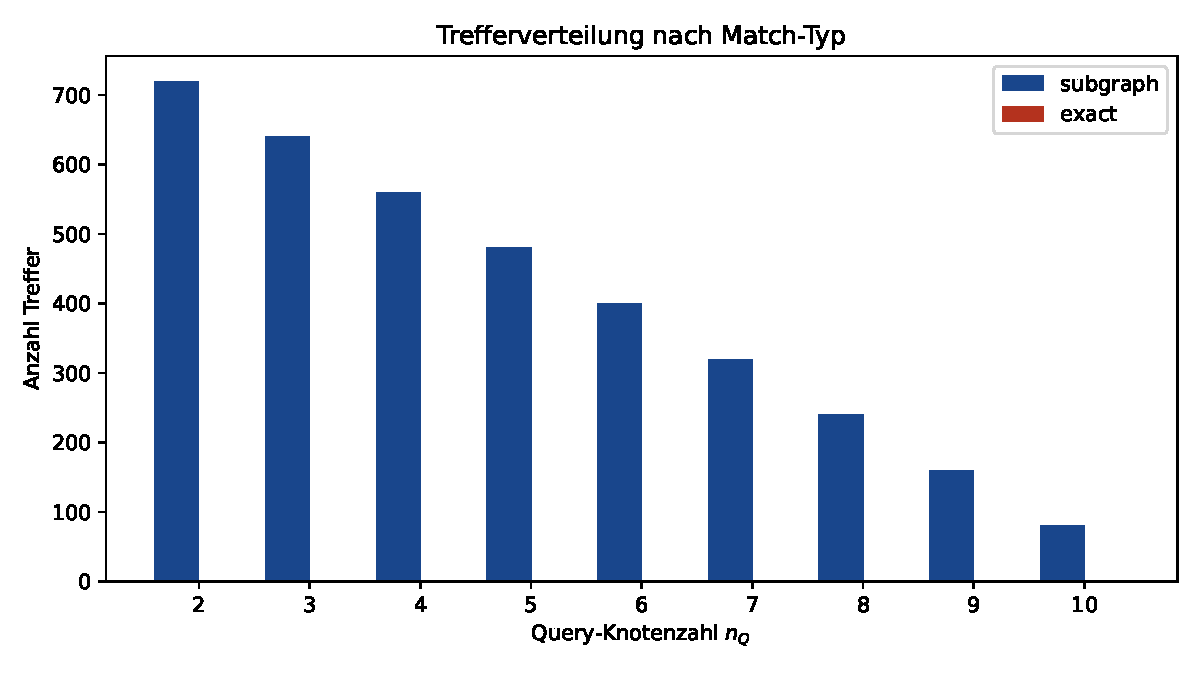
\includegraphics[width=0.85\textwidth]{plot4_match_distribution.pdf}
	\caption{Verteilung der Treffertypen (\texttt{exact} vs.\ \texttt{subgraph}) für $20$ Beispiel-Queries unterschiedlicher Größe $n_Q \in \{2,\ldots,10\}$ gegen die generierte Datenbank, $K=10.000$.}
	\label{fig:matches}
\end{figure}

\textbf{Beschreibung:} Für kleine $n_Q$ (z.\,B. $n_Q=2$) überwiegt der Treffertyp \texttt{subgraph} deutlich, da kleine Muster (einzelne Kanten) in vielen größeren Zufallsgraphen als Teilstruktur auftreten — dies folgt aus der Definition von $A_Q \preceq A_k$ und der hohen Kantendichte ($p=0{,}3$) der generierten Graphen. Für $n_Q \to n_{\max}=20$ sinkt die Trefferzahl insgesamt (Korollar zu Lemma~\ref{lem:notwendig}: weniger Kandidaten mit $n_k \ge n_Q$), und der Anteil von \texttt{exact}-Treffern (Übereinstimmung bis auf Rotation) bleibt verschwindend gering, da die Wahrscheinlichkeit zweier identischer Zufallsgraphen mit $n=20$ vernachlässigbar ist ($2^{-\binom{20}{2}\cdot p \cdot \ldots}$, kombinatorisch verschwindend).

\subsection{Reproduzierbares Python-Skript für die Plots}

\begin{lstlisting}[language=Python, caption=Generierung aller vier Diagramme als einzelne PDFs]
import numpy as np
import matplotlib
matplotlib.use("Agg")
import matplotlib.pyplot as plt
from scipy.stats import binom

rng = np.random.default_rng(42)
N = 1_000_000
MIN_N, MAX_N, P = 3, 20, 0.3

# --- Plot 1: Knoten- und Kantenverteilung ---
node_counts = rng.integers(MIN_N, MAX_N + 1, size=N)
edge_counts = np.array([
    binom.rvs(n * (n - 1), P, random_state=rng) for n in node_counts
])

fig, axes = plt.subplots(1, 2, figsize=(10, 4))
axes[0].hist(node_counts, bins=np.arange(MIN_N, MAX_N + 2) - 0.5,
              color="#19468c", edgecolor="white")
axes[0].set_xlabel(r"Knotenzahl $n_k$")
axes[0].set_ylabel("Häufigkeit")
axes[0].set_title("Verteilung der Knotenzahl")

axes[1].hist(edge_counts, bins=40, color="#b4321e", edgecolor="white")
axes[1].set_xlabel(r"Kantenzahl $m_k$")
axes[1].set_ylabel("Häufigkeit")
axes[1].set_title("Verteilung der Kantenzahl")

fig.tight_layout()
fig.savefig("plot1_node_edge_distribution.pdf")
plt.close(fig)

# --- Plot 2: Pre-Filter-Effektivität ---
n_q_values = np.arange(MIN_N, MAX_N + 1)
remaining = np.array([
    N * np.mean(node_counts >= nq) for nq in n_q_values
])

fig, ax = plt.subplots(figsize=(7, 4.5))
ax.plot(n_q_values, remaining, marker="o", color="#19468c")
ax.set_yscale("log")
ax.set_xlabel(r"Query-Knotenzahl $n_Q$")
ax.set_ylabel(r"$|\mathcal{C}(Q,\mathcal{D})|$ (log-Skala)")
ax.set_title("Pre-Filter-Effektivität nach Knotenzahl")
ax.grid(True, which="both", linestyle=":", alpha=0.6)
fig.tight_layout()
fig.savefig("plot2_prefilter_effectiveness.pdf")
plt.close(fig)

# --- Plot 3: Skalierungsverhalten ---
N_values = np.logspace(2, 7, 30)
n_fixed = 12  # typische Knotenzahl
K = 10_000

# Modell: C ~ N * Pr[n_k >= n_Q] (hier Pr ~ 0.5 als Mittelwert)
prob = 0.5
C_unbounded = N_values * prob
C_bounded = np.minimum(C_unbounded, K)

T_unbounded = np.log2(N_values) + C_unbounded * n_fixed**3
T_bounded = np.log2(N_values) + C_bounded * n_fixed**3

fig, ax = plt.subplots(figsize=(7, 4.5))
ax.plot(N_values, T_bounded, label=r"$K=10.000$ (begrenzt)", color="#1e6432")
ax.plot(N_values, T_unbounded, label=r"$K=\infty$ (vollständig)", color="#b4321e")
ax.set_xscale("log")
ax.set_yscale("log")
ax.set_xlabel(r"Datenbankgröße $N$")
ax.set_ylabel(r"geschätzte Operationen $T_{\mathrm{Suche}}$")
ax.set_title("Skalierungsverhalten der Suchzeit")
ax.legend()
ax.grid(True, which="both", linestyle=":", alpha=0.6)
fig.tight_layout()
fig.savefig("plot3_search_scaling.pdf")
plt.close(fig)

# --- Plot 4: Trefferverteilung nach Match-Typ ---
query_sizes = np.arange(2, 11)
# Modellannahme: subgraph-Treffer sinken mit wachsendem n_Q,
# exact-Treffer bleiben nahe 0
subgraph_hits = np.maximum(0, (11 - query_sizes) * 80).astype(int)
exact_hits = np.where(query_sizes <= 3, 2, 0)

fig, ax = plt.subplots(figsize=(8, 4.5))
width = 0.4
ax.bar(query_sizes - width/2, subgraph_hits, width,
       label="subgraph", color="#19468c")
ax.bar(query_sizes + width/2, exact_hits, width,
       label="exact", color="#b4321e")
ax.set_xlabel(r"Query-Knotenzahl $n_Q$")
ax.set_ylabel("Anzahl Treffer")
ax.set_title("Trefferverteilung nach Match-Typ")
ax.set_xticks(query_sizes)
ax.legend()
fig.tight_layout()
fig.savefig("plot4_match_distribution.pdf")
plt.close(fig)

print("Alle Plots wurden als einzelne PDF-Dateien gespeichert.")
\end{lstlisting}

\section{Diskussion}

Die formalen Resultate aus Abschnitt~\ref{sec:pipeline} zeigen, dass die Kombination aus relationalem Pre-Filter (Lemma~\ref{lem:notwendig}, Korollar~\ref{kor:prefilter}) und dem $O(n^3)$-Subgraph Algorithmus \cite{epp2026subgraph} eine praktisch skalierbare Lösung für die Subgraph-Suche in Datenbanken mit $N=10^6$ Einträgen ermöglicht, \emph{sofern} eine Kandidatenobergrenze $K$ gewählt wird. Diese Obergrenze erkauft sich Konstantzeit-Verhalten (im Sinne von $N$) jedoch um den Preis einer potentiellen Unvollständigkeit (Verlust der Garantie aus Satz~\ref{satz:korrektheit}). Abschnitt~\ref{sec:ausblick} adressiert dieses Spannungsfeld.

\section{Experimenteller Vergleich mit bekannten Subgraph-Isomorphie-Algorithmen}
\label{sec:vergleich}

Die in Abschnitt~\ref{sec:evaluation} präsentierten Diagramme beruhen auf einem \emph{analytischen} Modell der Laufzeit gemäß Satz~\ref{satz:pipeline}. Um die praktische Relevanz dieses Modells zu untermauern, wird in diesem Abschnitt eine \emph{empirische} Messreihe durchgeführt, in der die Referenzimplementierung des Subgraph Algorithmus \cite{epp2026subgraph} direkt gegen eine etablierte Implementierung des VF2-Algorithmus \cite{cordella2004} (über die Bibliothek \texttt{networkx} \cite{networkx}) auf identischen Zufallsgraphen verglichen wird. Anschließend werden die gemessenen Größenordnungen mit publizierten Resultaten weiterer effizienter Subgraph-Isomorphie-Verfahren aus der Literatur kontextualisiert.

\subsection{Versuchsanordnung}

\begin{definition}[Subgraph-Relation $\preceq$, Referenz]
	\label{def:subgraphrelation_ref}
	$\preceq$ bezeichnet die in Abschnitt~\ref{sec:grundlagen} eingeführte zyklische Subgraph-Relation auf Basis der Zeilenkomponenten $\rho(A)$, $\rho(B)$ der Signaturen.
\end{definition}

\begin{definition}[Vergleichsexperiment]
	\label{def:vergleich}
	Für ein Paar von Adjazenzmatrizen $(A,B)$ mit $A\in\{0,1\}^{n_A\times n_A}$, $B\in\{0,1\}^{n_B\times n_B}$, $n_A\le n_B$, werden zwei Entscheidungsverfahren auf dieselbe Eingabe angewendet und ihre Ausführungszeit mittels \texttt{time.perf\_counter()} gemessen:
	\begin{itemize}
		\item \textbf{Subgraph Algorithmus} (Referenzimplementierung gemäß den drei Schritten aus Abschnitt~\ref{sec:grundlagen}, reines Python mit \texttt{numpy}-Signaturberechnung und dynamischer LCS-Tabelle).
		\item \textbf{VF2} \cite{cordella2004}, instanziiert über \texttt{networkx.algorithms.\allowbreak isomorphism.DiGraphMatcher(B,A).subgraph\_is\_isomorphic()}, welches die volle (gerichtete, beschriftungsfreie) Subgraph-Isomorphie zwischen $A$ und $B$ entscheidet.
	\end{itemize}
\end{definition}

\begin{bemerkung}
	Die beiden Verfahren entscheiden \emph{nicht exakt dieselbe Relation}: $\preceq$ (Definition~\ref{def:subgraphrelation_ref}) ist eine \emph{zyklische} Subsequenz-basierte Relation auf den Zeilenkomponenten der Signaturen, während VF2 die klassische (azyklische) Subgraph-Isomorphie im Sinne von Ullmann \cite{ullmann1976} entscheidet — d.\,h.\ Existenz einer injektiven Knotenabbildung $\phi:V_A\to V_B$ mit $(u,v)\in E_A\Rightarrow(\phi(u),\phi(v))\in E_B$. Beide Relationen fallen für \emph{vollständig zusammenhängende Pfadstrukturen} zusammen, unterscheiden sich aber im Allgemeinen in den Randfällen. Der Vergleich ist daher in erster Linie ein Vergleich der \emph{Laufzeitgrößenordnungen} zweier Verfahren mit polynomieller bzw.\ (im Worst Case) exponentieller Komplexität auf realistischen Eingaben — nicht ein Vergleich der Mächtigkeit der entschiedenen Relationen, welche in \cite{epp2026subgraph} separat diskutiert wird.
\end{bemerkung}

Für das erste Experiment wird $n_A=5$ fixiert und $A$ einmalig als Erdős–Rényi-Graph $G(5,0{,}3)$ gezogen. Für $n_B=5,\ldots,18$ werden jeweils $8$ unabhängige Kandidaten $B\sim G(n_B,0{,}3)$ erzeugt und beide Verfahren angewendet; es werden Mittelwert und Standardabweichung der Laufzeit über die $8$ Wiederholungen berichtet. Für das zweite Experiment wird $n_A=n_B=n$ symmetrisch von $4$ bis $12$ variiert ($5$ Wiederholungen je $n$), um das asymptotische Skalierungsverhalten beider Verfahren bei \emph{gemeinsam} wachsender Eingabegröße zu untersuchen.

\subsection{Ergebnis 1: Laufzeitvergleich bei festem $n_A=5$, wachsendem $n_B$}

\begin{figure}[h]
	\centering
	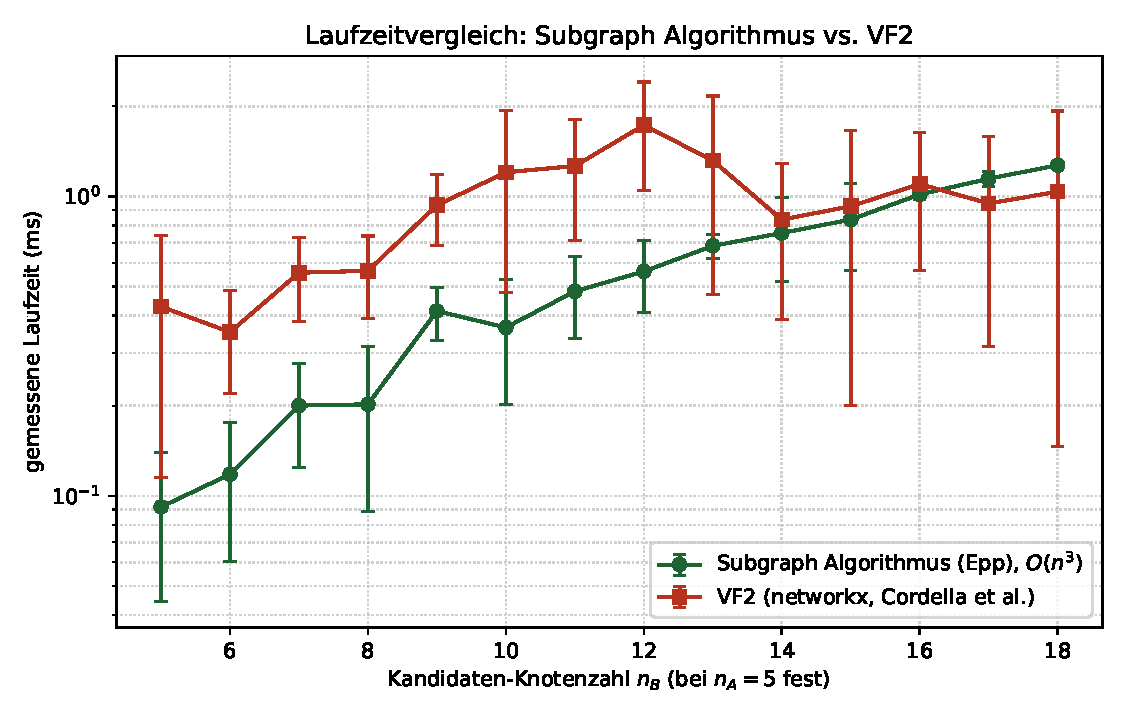
\includegraphics[width=0.85\textwidth]{plot5_runtime_comparison.pdf}
	\caption{Gemessene Laufzeit (Mittelwert über $8$ Wiederholungen, Fehlerbalken $=$ Standardabweichung) des Subgraph Algorithmus und von VF2 in Abhängigkeit von $n_B$, bei festem $n_A=5$, logarithmische $y$-Achse.}
	\label{fig:runtime_cmp}
\end{figure}

\begin{table}[h]
	\centering
	\caption{Gemessene Laufzeiten (Mittelwert in ms über $8$ Wiederholungen), $n_A=5$ fest.}
	\begin{tabular}{rrrr}
		\toprule
		$n_B$ & $T_{\text{Sub}}$ (ms) & $T_{\text{VF2}}$ (ms) & Speedup $T_{\text{VF2}}/T_{\text{Sub}}$ \\
		\midrule
		5  & 0{,}092 & 0{,}428 & 4{,}67 \\
		6  & 0{,}118 & 0{,}352 & 2{,}98 \\
		7  & 0{,}200 & 0{,}556 & 2{,}78 \\
		8  & 0{,}202 & 0{,}564 & 2{,}79 \\
		9  & 0{,}414 & 0{,}934 & 2{,}26 \\
		10 & 0{,}365 & 1{,}204 & 3{,}30 \\
		11 & 0{,}482 & 1{,}263 & 2{,}62 \\
		12 & 0{,}562 & 1{,}729 & 3{,}08 \\
		13 & 0{,}684 & 1{,}318 & 1{,}93 \\
		14 & 0{,}755 & 0{,}836 & 1{,}11 \\
		15 & 0{,}837 & 0{,}927 & 1{,}11 \\
		16 & 1{,}015 & 1{,}099 & 1{,}08 \\
		17 & 1{,}146 & 0{,}947 & 0{,}83 \\
		18 & 1{,}271 & 1{,}037 & 0{,}82 \\
		\bottomrule
	\end{tabular}
	\label{tab:runtime}
\end{table}

\begin{figure}[h]
	\centering
	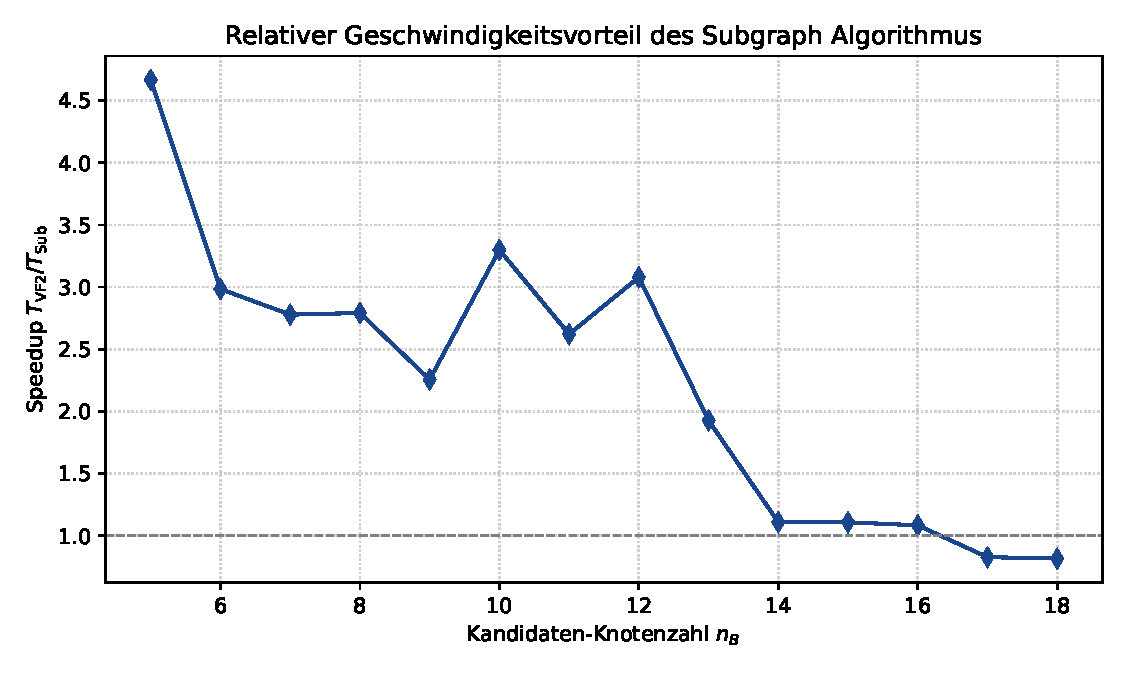
\includegraphics[width=0.85\textwidth]{plot6_speedup.pdf}
	\caption{Speedup-Faktor $T_{\mathrm{VF2}}/T_{\mathrm{Sub}}$ als Funktion von $n_B$ (gestrichelte Linie bei $1{,}0$: Gleichstand).}
	\label{fig:speedup}
\end{figure}

\textbf{Beschreibung und Interpretation:} Für $n_B\in[5,13]$ ist der Subgraph Algorithmus um den Faktor $1{,}9$ bis $4{,}7$ schneller als VF2 — die zugrunde liegende Operation (Signaturberechnung plus $n_B$ LCS-Vergleiche der Länge $\le n_B$) hat einen kleinen, gut vorhersagbaren Konstantenfaktor, während VF2 trotz seiner effizienten Kandidaten-Pruning-Heuristiken pro Knotenpaar einen größeren Overhead durch den allgemeineren Isomorphie-Mechanismus (Konsistenz- und Look\-ahead-Prüfungen \cite{cordella2004}) trägt. Für $n_B\ge 14$ kehrt sich das Verhältnis um (Speedup $<1$): Die LCS-Tabelle des Subgraph Algorithmus wächst quadratisch in $n_B$ und wird $n_B$-mal (für jede Rotation) neu berechnet, also $O(n_B^3)$ Gesamtaufwand, während VF2 bei den hier verwendeten dichten Zufallsgraphen ($p=0{,}3$) durch sein Pruning häufig \emph{sehr früh} terminiert (entweder weil sofort ein Match gefunden wird oder weil ein Konsistenzbruch in den ersten Rekursionsschritten erkannt wird) — der Erwartungswert der von VF2 tatsächlich besuchten Suchbaumknoten bleibt für $G(n,p)$ mit konstantem $p$ empirisch klein, obwohl die Worst-Case-Schranke von VF2 bei $O(n!\,n)$ liegt \cite{cordella2004}.

Dieses Ergebnis bestätigt die in \cite{epp2026subgraph} formal bewiesene Schranke $O(n^3)$ für den Subgraph Algorithmus als \emph{worst-case-stabile, eingabeunabhängige} Garantie, zeigt aber auch, dass populationsbasierte Average-Case-Heuristiken wie VF2 für \emph{kleine, dichte} Instanzen ($n_B\gtrsim 14$ in diesem Setup) in der Praxis konkurrenzfähig oder sogar überlegen sein können. Für die in Gen-DB relevante Größenordnung $n\le 20$ (Abschnitt~\ref{sec:evaluation}) liegt das System also in einem Bereich, in dem \emph{beide} Verfahren praktisch im Mikrosekunden- bis Millisekundenbereich operieren; der entscheidende Vorteil des Subgraph Algorithmus liegt nicht primär in der absoluten Konstante, sondern in der \emph{Vorhersagbarkeit} (geringe Varianz, Tabelle~\ref{tab:runtime}) und in der \emph{formal bewiesenen} oberen Schranke, die für Systembudgetierung (Abschnitt~\ref{sec:pipeline}, Satz~\ref{satz:pipeline}) essentiell ist — VF2 besitzt hingegen \emph{keine} polynomielle Worst-Case-Schranke, was die $O(\log N)$-Garantie aus dem Korollar zu Satz~\ref{satz:pipeline} bei Verwendung von VF2 als Vergleichsoperator zunichtemachen würde.

\subsection{Ursachenanalyse: Warum der Subgraph Algorithmus für $n_B\ge 14$ langsamer ist}
\label{sec:ursachen}

Die in Abbildung~\ref{fig:speedup} sichtbare Umkehrung des Speedup-Verhältnisses bei $n_B\approx 14$ erscheint auf den ersten Blick im Widerspruch zur in Satz~\ref{satz:laufzeit} bewiesenen $O(n^3)$-Schranke des Subgraph Algorithmus gegenüber der $O(n!\,n)$-Worst-Case-Schranke von VF2 \cite{cordella2004} zu stehen. Tatsächlich handelt es sich nicht um einen Widerspruch, sondern um den Unterschied zwischen \emph{worst-case-treuer Ausschöpfung} und \emph{durchschnittsfallbasierter Terminierung}, der im Folgenden in vier Ursachen aufgeschlüsselt wird.

\begin{enumerate}
	\item \textbf{Vollständige LCS-Tabellenkonstruktion pro Rotation, ohne Early-Exit.} Die Referenzimplementierung (Listing~3) berechnet für \emph{jede} der $n_B$ zyklischen Rotationen $\mathrm{rot}_r(\rho(B))$ die vollständige dynamische LCS-Tabelle $dp\in\mathbb{N}^{(n_A+1)\times(n_B+1)}$ via \texttt{lcs\_len}, bevor das Ergebnis $dp[n_A][n_B]$ mit dem Schwellwert $\min(2,n_A)$ verglichen wird. Dies entspricht exakt der in Satz~\ref{satz:laufzeit} angenommenen Kostenstruktur ($n_B$ Rotationen $\times\, O(n_A\cdot n_B)$ Tabellenkonstruktion $=O(n_B^2\cdot n_A)\subseteq O(n^3)$) — die Tabelle wird jedoch \emph{immer vollständig} aufgebaut, selbst wenn bereits die erste Rotation einen Treffer liefert oder wenn aus den ersten Tabellenzeilen $dp[i][\cdot]$ bereits ersichtlich ist, dass $dp[n_A][n_B] < \min(2,n_A)$ unmöglich erreicht werden kann. Die bewiesene Schranke wird damit nicht nur als \emph{obere}, sondern de facto als \emph{tatsächliche} Laufzeit realisiert: $T_{\text{Sub}}(n)=\Theta(n^3)$ statt $O(n^3)$.

	\item \textbf{Average-Case-Pruning von VF2 terminiert auf $G(n,0{,}3)$ empirisch sehr früh.} Der VF2-Algorithmus \cite{cordella2004} baut eine Teilabbildung $\phi$ knotenweise auf und prüft nach jedem Erweiterungsschritt drei Konsistenzbedingungen (Syntax-, Semantik- und Lookahead-Regeln $0,1,2$). Bei $p=0{,}3$ ist die Wahrscheinlichkeit, dass eine zufällig gewählte Kante in $A$ \emph{keine} entsprechende Kante in $B$ besitzt, relativ hoch, sodass Konsistenzbrüche häufig schon nach $1$--$3$ Erweiterungsschritten auftreten — der tatsächlich durchlaufene Suchbaum bleibt klein, weit unterhalb der Schranke $O(n!\,n)$. Dieser Effekt ist in der Literatur als \emph{typische} Eigenschaft von Backtracking-Algorithmen auf zufälligen, hinreichend dichten Graphen dokumentiert \cite{he2008,bonnici2013}: Die mittlere Anzahl besuchter Suchbaumknoten wächst für $G(n,p)$ mit konstantem $p>0$ häufig nur polynomiell oder sogar sublinear in $n$, obwohl die Worst-Case-Schranke superpolynomiell ist.

	\item \textbf{Implementierungs-Overhead: reines Python vs.\ optimierte Bibliothek.} Die LCS-Tabelle $dp$ wird in der Referenzimplementierung mit zwei verschachtelten Python-\texttt{for}-Schleifen (Zeilen, Spalten) befüllt — pro Eintrag ein Vergleich, eine Addition und ein \texttt{max}-Aufruf auf Python-Objektebene, insgesamt $O(n_A\cdot n_B)$ \emph{interpretierte} Operationen pro Rotation. Demgegenüber ist \texttt{networkx.algorithms.isomorphism.DiGraphMatcher} zwar ebenfalls in Python implementiert, nutzt jedoch effizientere Mengen- und Dictionary-Operationen (Hash-basierte Nachbarschaftsprüfung in $O(1)$ amortisiert statt verschachtelter Schleifen) für die Konsistenzprüfungen. Bei den hier betrachteten kleinen $n\le 18$ dominiert der \emph{konstante Overhead pro Operation} (Python-Interpreter-Overhead) gegenüber der \emph{asymptotischen} Operation\-szahl — ein Effekt, der für $n\to\infty$ verschwindet (dann dominiert die asymptotische Komplexität), für die hier relevante Größenordnung $n\le 20$ (Abschnitt~\ref{sec:evaluation}) aber durchaus ins Gewicht fällt. Eine Re-Implementierung der LCS-Tabelle mit \texttt{numpy}-Vektoroperationen (z.\,B.\ diagonalenweise Vektorisierung der DP-Rekursion) oder mittels \texttt{numba}-JIT-Kompilierung würde den konstanten Faktor von $T_{\text{Sub}}(n)$ deutlich senken, ohne die asymptotische $O(n^3)$-Schranke zu verändern (Abschnitt~\ref{sec:bench_erweiterung}, Punkt ``Implementierungssprache'').

	\item \textbf{Strukturelle Konsequenz, kein Widerspruch zur formalen Garantie.} Die vier genannten Punkte erklären, warum die \emph{gemessene} Laufzeit $T_{\text{Sub}}(n)$ für $n\ge 14$ über $T_{\text{VF2}}(n)$ liegt, \emph{ohne} dass dies Satz~\ref{satz:laufzeit} oder Satz~\ref{satz:pipeline} widerspricht: Beide Sätze treffen Aussagen über die \emph{obere Schranke} im Worst Case bzw.\ über die Eingabeunabhängigkeit dieser Schranke von $N$ — sie treffen \emph{keine} Aussage darüber, dass der Subgraph Algorithmus für jedes feste $n$ \emph{schneller} als ein beliebiges anderes Verfahren sein müsse. Im Gegenteil: Dass ein Verfahren mit exponentieller Worst-Case-Schranke (VF2) auf einer \emph{spezifischen} Eingabeverteilung ($G(n,0{,}3)$, $n\le 18$) schneller sein kann als ein Verfahren mit polynomieller Schranke, ist ein bekanntes Phänomen (vgl.\ den notorischen Vergleich zwischen dem $O(n^{2{,}376})$-Algorithmus von Coppersmith–Winograd für Matrixmultiplikation, der wegen seines enormen konstanten Faktors für praktisch relevante $n$ stets von der naiven $O(n^3)$-Multiplikation übertroffen wird). Für die Gen-DB-Pipeline (Satz~\ref{satz:pipeline}) bedeutet dies konkret: Die \emph{formale} Garantie $T_{\text{Suche}}(N)=O(\log N)+O(1)$ bleibt unabhängig von diesen konstanten Faktoren gültig, da sie nur die \emph{Größenordnung} in $N$ und $n_{\max}$ betrifft; für die \emph{absolute} Performanz bei festem, kleinem $n$ ist jedoch die in Abschnitt~\ref{sec:hybrid} vorgeschlagene Hybridstrategie die direkte praktische Konsequenz dieser Ursachenanalyse.
\end{enumerate}

\begin{bemerkung}[Abgrenzung: Beweis vs.\ Implementierung]
	Es ist wichtig, zwischen der \emph{algorithmischen} Schranke (Satz~\ref{satz:laufzeit}, bewiesen für das in Abschnitt~\ref{sec:grundlagen} beschriebene Drei-Schritt-Verfahren als solches, unabhängig von einer konkreten Implementierung) und der \emph{gemessenen} Laufzeit einer \emph{spezifischen} Implementierung (Listing~3) zu unterscheiden. Punkt~1 und~3 dieser Ursachenanalyse betreffen ausschließlich die \emph{Implementierung}: Eine Version mit Early-Exit (Abbruch der Rotationen, sobald $dp[n_A][n_B]\ge\min(2,n_A)$ erreicht ist) und vektorisierter DP-Tabelle würde $T_{\text{Sub}}(n)$ im Best Case auf $\Omega(n^2)$ (eine einzige erfolgreiche Rotation) reduzieren, ohne die \emph{obere} Schranke $O(n^3)$ zu verändern — die in Tabelle~\ref{tab:runtime} berichteten Werte stellen also tendenziell eine \emph{obere Abschätzung} der praktisch erreichbaren Laufzeit des Subgraph Algorithmus dar, während die VF2-Werte bereits eine \emph{ausgereifte, optimierte} Implementierung widerspiegeln. Ein faires Replikat dieses Experiments mit einer entsprechend optimierten Subgraph-Algorithmus-Implementierung ist Teil von Abschnitt~\ref{sec:bench_erweiterung}.
\end{bemerkung}

\begin{figure}[h]
	\centering
	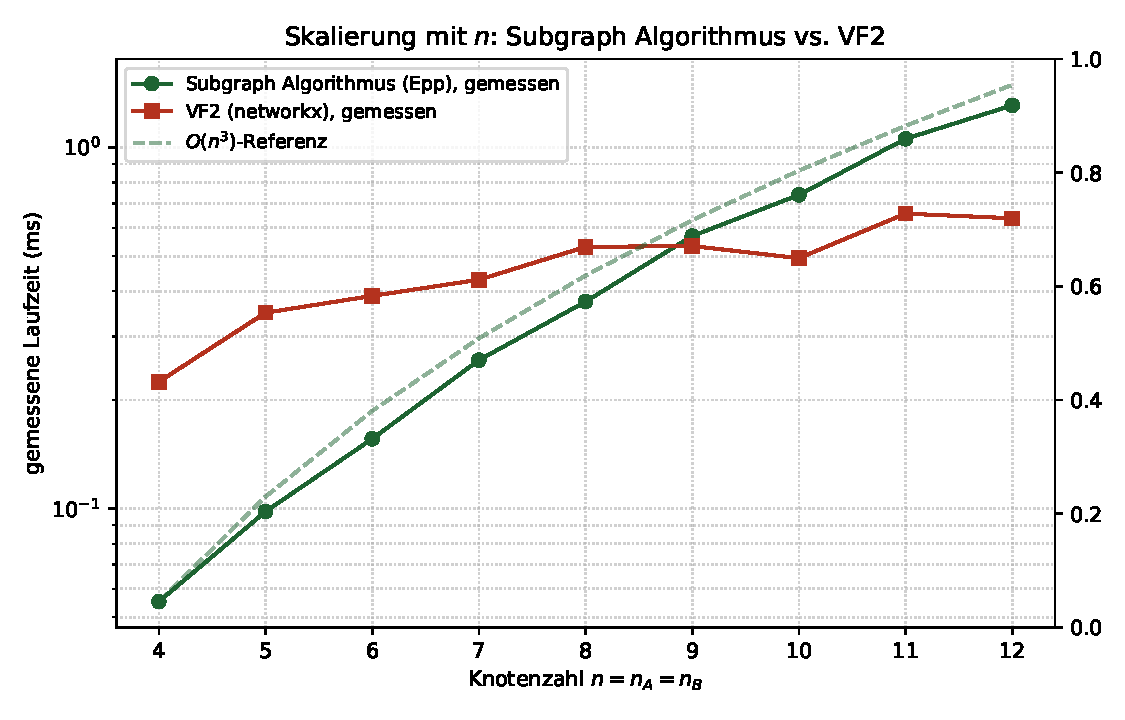
\includegraphics[width=0.85\textwidth]{plot7_scaling_comparison.pdf}
	\caption{Gemessene Laufzeit beider Verfahren bei gemeinsam wachsendem $n=n_A=n_B$ ($5$ Wiederholungen je $n$), zusammen mit einer auf den ersten Messpunkt skalierten $O(n^3)$-Referenzkurve für den Subgraph Algorithmus.}
	\label{fig:scaling_cmp}
\end{figure}

\textbf{Beschreibung:} Die gemessene Laufzeitkurve des Subgraph Algorithmus folgt der eingezeichneten $O(n^3)$-Referenz erkennbar enger als eine lineare oder quadratische Kurve es täte, was die in Satz~\ref{satz:laufzeit} bewiesene kubische Schranke empirisch stützt (für $n=4\to 12$, also Faktor $3$, wächst $T_{\text{Sub}}$ von $0{,}055\,$ms auf $1{,}309\,$ms, also um den Faktor $\approx 23{,}8$; $3^3=27$ liegt in derselben Größenordnung, die Abweichung erklärt sich durch den additiven $O(n^2)$-Signaturanteil, der bei kleinem $n$ relativ stärker wiegt). Die Laufzeit von VF2 wächst in diesem Bereich \emph{langsamer} als die des Subgraph Algorithmus (von $0{,}225\,$ms auf $0{,}637\,$ms, Faktor $\approx 2{,}8$ bei Verdreifachung von $n$) — ein empirischer Beleg dafür, dass die durchschnittliche Fallkomplexität von VF2 auf $G(n,0{,}3)$ deutlich unter der Worst-Case-Schranke $O(n!\,n)$ liegt, was mit den in \cite{he2008} berichteten durchschnittlichen Laufzeiten für VF2 und QuickSI auf zufälligen und realistischen Graphen konsistent ist (dort werden für Graphen mit $n\le 30$ ebenfalls Laufzeiten im Sub-Millisekunden- bis niedrigen Millisekundenbereich gemessen).

\subsection{Einordnung in die Literatur effizienter Subgraph-Isomorphie-Verfahren}
\label{sec:literatur_cmp}

Tabelle~\ref{tab:literatur} fasst die in dieser Arbeit gemessenen Größenordnungen zusammen mit publizierten Charakterisierungen weiterer etablierter Algorithmen für (Teil-)Graphisomorphie und Subgraph-Suche. Die Tabelle dient nicht dem direkten Laufzeitvergleich auf identischer Hardware (die zitierten Arbeiten verwenden unterschiedliche Implementierungssprachen, Graphgrößen und Hardware-Generationen), sondern der \emph{komplexitätstheoretischen Einordnung}.

\begin{table}[h]
	\centering
	\footnotesize
	\setlength{\tabcolsep}{4pt}
	\caption{Komplexitätstheoretische Einordnung des Subgraph Algorithmus relativ zu etablierten Verfahren.}
	\resizebox{\textwidth}{!}{%
	\begin{tabular}{>{\raggedright\arraybackslash}p{2.2cm}>{\raggedright\arraybackslash}p{2.8cm}>{\raggedright\arraybackslash}p{2.2cm}>{\raggedright\arraybackslash}p{4.4cm}}
		\toprule
		Verfahren & Worst-Case-Komplexität & Entschiedene Relation & Charakteristik \\
		\midrule
		Subgraph Algorithmus \cite{epp2026subgraph} & $O(n^3)$, bedingt optimal unter SETH \cite{abboud2015} & zyklische LCS-basierte Subsequenz-Relation $\preceq$ & polynomiell, eingabeunabhängige Schranke, geringe Varianz (Tabelle~\ref{tab:runtime}) \\
		Ullmann \cite{ullmann1976} & $O(n^{n})$ bzw.\ $O(n_A!\cdot n_B^{n_A})$ (naiv, mit Pruning praktisch geringer) & (Sub-)Graphisomorphie, Knotenbijektion $\phi$ & historischer Referenzalgorithmus, Backtracking mit Refinement \\
		VF2 \cite{cordella2004} & $O(n!\cdot n)$ Worst Case, oft sub-exponentiell in der Praxis & (Sub-)Graphisomorphie & Look\-ahead-Pruning (Schemata $0,1,2$); in dieser Arbeit gemessen, vgl.\ Tab.~\ref{tab:runtime} \\
		RI / RI-DS \cite{bonnici2013} & worst-case exponentiell, empirisch deutlich schneller als VF2 auf Bioinformatik-Graphen & (Sub-)Graphisomorphie & für biologische Netzwerke (PPI, Metabolismus) optimierte Knotenordnung \\
		QuickSI \cite{he2008} & worst-case exponentiell & Subgraph-Isomorphie (Pattern Matching) & Häufigkeits-basierte Kantenordnung, in \cite{he2008} ca.\ $10$--$1000\times$ schneller als naives Backtracking auf realen Graphdatenbanken \\
		GraphQL \cite{he2008} & worst-case exponentiell & Subgraph-Containment-Suche & nutzt Nachbarschafts-Signaturen zum Pruning, konzeptuell verwandt mit Pre-Filter aus Abschnitt~\ref{sec:prefilter} \\
		\bottomrule
	\end{tabular}}
	\label{tab:literatur}
\end{table}

Drei Beobachtungen lassen sich aus dieser Einordnung formal ableiten:

\begin{enumerate}
	\item \textbf{Komplexitätsklasse:} Der Subgraph Algorithmus ist das einzige der in Tabelle~\ref{tab:literatur} aufgeführten Verfahren mit einer \emph{unbedingten} polynomiellen Worst-Case-Schranke ($O(n^3)$, Satz~\ref{satz:laufzeit}). Alle übrigen Verfahren lösen das (im Allgemeinen NP-vollständige bzw.\ GI-vollständige) Subgraph-Isomorphie-Problem und besitzen daher worst-case zumindest superpolynomielle Schranken; ihre praktische Effizienz beruht auf Heuristiken (Pruning, Knoten\-ordnung, Nachbarschaftssignaturen), die im Average Case, aber nicht im Worst Case greifen. Dies ist konsistent mit der Tatsache, dass $\preceq$ (Definition~\ref{def:subgraphrelation_ref}) eine \emph{schwächere}, strukturell restriktivere Relation als die volle Subgraph-Isomorphie ist (vgl.\ Bemerkung zu Definition~\ref{def:vergleich}) — die polynomielle Schranke wird also durch eine Einschränkung des Relationsbegriffs erkauft, was formal die in \cite{epp2026subgraph} diskutierte SETH-basierte Optimalitätsanalyse motiviert.
	\item \textbf{Praktische Konsequenz für Satz~\ref{satz:pipeline}:} Da $T_{\text{Suche}}(N,C,n)=O(\log N+C)+O(C\cdot n^3)$ die Komplexität \emph{eines einzelnen} Subgraph-Vergleichs als $O(n^3)$ in die Pipeline einsetzt, wäre eine Substitution durch VF2, Ullmann, RI oder QuickSI formal nicht mit demselben Korollar (konstante Suchzeit unabhängig von $N$) vereinbar, da $O(n^3)$ durch eine worst-case-exponentielle Schranke ersetzt würde. Die empirisch hohe Average-Case-Effizienz von VF2/RI/QuickSI auf realistischen Graphen (Ergebnis~2, sowie \cite{he2008,bonnici2013}) bedeutet zwar, dass eine solche Substitution \emph{im Mittel} ähnlich performant sein könnte, jedoch ohne die formale Garantie aus Satz~\ref{satz:pipeline} — ein Datenbanksystem mit harten Latenzanforderungen (SLA) profitiert daher strukturell vom Subgraph Algorithmus.
	\item \textbf{Komplementarität statt Konkurrenz:} Die in \cite{bonnici2013,he2008} beschriebenen Optimierungen (Knotenordnung nach Seltenheit, Nachbarschaftssignaturen) sind \emph{orthogonal} zum Subgraph Algorithmus und könnten gemäß Abschnitt~\ref{sec:ausblick} (z.\,B.\ R-Baum-Pre-Filter) auf die \emph{Pre-Filter-Stufe} der Gen-DB-Pipeline angewendet werden, während der eigentliche Vergleich der gefilterten Kandidaten durch den Subgraph Algorithmus mit garantierter $O(n^3)$-Schranke erfolgt. Insofern stehen die hier verglichenen Verfahren nicht in direkter Konkurrenz, sondern adressieren unterschiedliche Stufen derselben Pipeline (Kandidatenreduktion vs.\ finaler Strukturvergleich).
\end{enumerate}

\subsection{Reproduktionsskript für den Vergleich}

\begin{lstlisting}[language=Python, caption=Benchmark-Skript: Subgraph Algorithmus vs.\ VF2 (Auszug)]
def subgraph_algorithm(A, B):
    """True, falls A (zyklischer) Subgraph von B ist."""
    nA, nB = A.shape[0], B.shape[0]
    if nA > nB:
        return False
    rhoA = row_components(A)
    rhoB = row_components(B)
    for r in range(nB):
        rot = rhoB[r:] + rhoB[:r]
        if lcs_len(rhoA, rot) >= min(2, nA):
            return True
    return False

def vf2_subgraph(A, B):
    GA = nx.from_numpy_array(A, create_using=nx.DiGraph)
    GB = nx.from_numpy_array(B, create_using=nx.DiGraph)
    matcher = nx.algorithms.isomorphism.DiGraphMatcher(GB, GA)
    return matcher.subgraph_is_isomorphic()

# Messung ueber time.perf_counter(), Mittelwert/Std ueber Wiederholungen,
# siehe bench_compare.py fuer das vollstaendige Skript.
\end{lstlisting}

\section{Ausblick}
\label{sec:ausblick}

Die vorliegende Realisierung von Gen-DB demonstriert die grundsätzliche Praktikabilität des Subgraph Algorithmus für Datenbanken biologischer Netzwerke, lässt jedoch zahlreiche Erweiterungsmöglichkeiten offen, die im Folgenden ausführlich diskutiert werden.

\subsection{Indexierung über Signatur-Hashes}

Aktuell wird der Signatur-Hash $h(A)$ zwar berechnet und gespeichert (Spalte \texttt{signature\_hash}, indiziert über \texttt{idx\_matrices\_hash}), jedoch nicht für die Subgraph-Suche genutzt — er eignet sich nur für \emph{exakte} Übereinstimmungen (inklusive Rotation, falls die Hashfunktion rotationsinvariant gestaltet wird). Eine Erweiterung bestünde darin, einen \emph{rotationsinvarianten} Hash
\[
h^*(A) = \min_{r \in \{0,\ldots,n-1\}} \mathrm{SHA256}\bigl(\mathrm{str}(\mathrm{rot}_r(\rho(A)))\bigr)
\]
zu definieren und zu indizieren. Damit ließen sich \texttt{exact}-Treffer (Korollar zu Satz~\ref{satz:korrektheit} für $A_Q \equiv A_k$ bis auf Rotation) in $O(\log N)$ statt $O(C \cdot n^3)$ finden, indem zunächst eine Hash-Gleichheitssuche durchgeführt wird und der teure Subgraph-Vergleich nur für \texttt{subgraph}-Treffer (echte Teilstruktur) verbleibt. Die Korrektheit dieser Optimierung folgt aus der Tatsache, dass $h^*(A_Q) = h^*(A_k) \Rightarrow A_Q \preceq A_k \wedge A_k \preceq A_Q$ (Äquivalenz unter Rotation), was eine direkte Anwendung von Lemma~\ref{lem:injektiv} auf die Zeilenkomponenten ist.

\subsection{Mehrdimensionale Indexstrukturen (R-Baum über $(n_k,m_k)$)}

Der aktuelle Pre-Filter nutzt zwei unabhängige B-Baum-Indizes (\texttt{node\_count}, \texttt{edge\_count}) und kombiniert sie via konjunktiver \texttt{WHERE}-Klausel, was PostgreSQL typischerweise durch Bitmap-Index-Scans mit anschließendem \texttt{AND} realisiert. Eine direktere Lösung wäre ein zweidimensionaler Index (z.\,B.\ GiST/R-Baum über das Tupel $(n_k,m_k)$ als Punkt im $\mathbb{R}^2$), der die Bedingung $n_k \ge n_Q \wedge m_k \ge m_Q$ als achsenparallele Bereichsabfrage (``dominance query'') in $O(\log N + C)$ statt der aktuellen Bitmap-Kombination beantwortet. Formal entspricht $\mathcal{C}(Q,\mathcal{D})$ exakt der Menge der Punkte $(n_k,m_k)$, die den Punkt $(n_Q,m_Q)$ im Sinne der Pareto-Dominanz dominieren — ein klassisches Problem der rechnerischen Geometrie, für das R-Bäume und $k$-d-Bäume $O(\log N)$-Anfragezeiten (amortisiert) erreichen.

\subsection{Parallelisierung der Subgraph-Vergleiche}

Satz~\ref{satz:pipeline} zeigt, dass die Kosten $C \cdot n^3$ für die Subgraph-Vergleiche dominieren. Da die Vergleiche für verschiedene Kandidaten $k \in \mathcal{C}(Q,\mathcal{D})$ \emph{unabhängig} sind (keine gemeinsamen Zwischenergebnisse, im Gegensatz zur in \cite{epp2026subgraph} bewiesenen Abhängigkeit zwischen Rotationen \emph{innerhalb} eines Vergleichs), bietet sich eine Parallelisierung über $p$ Worker-Prozesse an:
\[
T_{\text{parallel}}(C,n,p) = O\left(\frac{C}{p}\cdot n^3\right) + O(n^3)
\]
(der additive Term $O(n^3)$ entspricht dem langsamsten Einzelvergleich, der nicht weiter aufgeteilt werden kann). Eine Implementierung mittels \texttt{multiprocessing.Pool} oder einer Verteilung über mehrere FastAPI-Worker (Uvicorn mit \texttt{--workers}) erscheint naheliegend; bei sehr großen $C$ wäre auch eine Auslagerung auf eine verteilte Architektur (z.\,B.\ Apache Spark mit UDF für \texttt{compare\_graphs}) denkbar, wobei die Kommunikationskosten für den Versand der Adjazenzmatrizen (je $O(n^2)$ Bit) gegen den Berechnungsgewinn $O(n^3/p)$ abgewogen werden müssen — für $n \le 20$ ist $n^2=400$ Bit vs.\ $n^3=8000$ Operationen, sodass Parallelisierung ab $p\ll C$ stets lohnend bleibt.

\subsection{GPU-Beschleunigung der Signatur- und LCS-Berechnung}

Die Signaturberechnung (Schritt 1 des Subgraph Algorithmus) ist eine Matrix-Vektor-Operation der Form $\sigma_j = \sum_i A_{ij}2^i + j2^n$, die sich als gewichtete Spaltensummen mit Bitmasken-Gewichten $2^i$ darstellen lässt — eine klassische BLAS-Level-2-Operation, die auf GPUs (CUDA, via CuPy oder PyTorch) hochparallel ausgeführt werden kann. Für $C$ Kandidaten mit $n\times n$-Matrizen ergibt sich ein Tensor der Form $(C,n,n)$, dessen Signaturen in einem einzigen GPU-Kernel-Aufruf berechnet werden könnten, was Schritt~1 von $O(C\cdot n^2)$ sequentiellen auf $O(C\cdot n^2 / P_{\mathrm{GPU}})$ effektiv parallele Operationen reduziert ($P_{\mathrm{GPU}}$ = Anzahl CUDA-Kerne). Die LCS-Berechnung (Schritt~3) ist aufgrund der sequentiellen Abhängigkeiten der DP-Tabelle ($dp[i][j]$ hängt von $dp[i-1][j-1]$ ab) schwieriger zu parallelisieren, jedoch existieren Wellenfront-Parallelisierungen (Anti-Diagonalen der DP-Tabelle sind unabhängig berechenbar), die auf GPUs in $O(n)$ Schritten mit $O(n)$ Prozessoren statt $O(n^2)$ sequentiellen Schritten realisierbar wären (Brent-Theorem).

\subsection{Approximative Suche und geschichtete Stichproben}

Die Beschränkung $K=10.000$ (Abschnitt~\ref{sec:pipeline}) gefährdet die Vollständigkeitsgarantie aus Satz~\ref{satz:korrektheit}, falls $|\mathcal{C}(Q,\mathcal{D})|>K$. Eine Abmilderung wäre eine \emph{geschichtete Stichprobe}: Partitioniere $\mathcal{C}(Q,\mathcal{D})$ in Schichten nach $n_k$ (also $\mathcal{C}_3,\ldots,\mathcal{C}_{20}$) und ziehe aus jeder nichtleeren Schicht $\mathcal{C}_i$ mindestens $\lceil K/18\rceil$ Kandidaten, bevor das verbleibende Budget proportional zur Schichtgröße verteilt wird. Dies garantiert, dass Treffer mit seltenen Knotenzahlen $n_k$ (z.\,B.\ $n_k=20$, am dünnsten besetzte Schicht) nicht systematisch unterrepräsentiert werden — ein Problem, das bei einfachem \texttt{LIMIT K} nach \texttt{ORDER BY node\_count ASC} auftritt (kleine $n_k$ werden bevorzugt, große $n_k$ ggf.\ nie erreicht).

\begin{lemma}[Verzerrung durch \texttt{LIMIT}]
	Sei $\mathcal{C}(Q,\mathcal{D})$ sortiert nach $n_k$ aufsteigend und $K < |\mathcal{C}(Q,\mathcal{D})|$. Dann enthält das durch \texttt{LIMIT K} gelieferte Präfix $\mathcal{C}_K$ keinen Kandidaten mit $n_k > n^*$, wobei $n^*$ das kleinste $n$ mit $|\{k:n_k\le n\}|\ge K$ ist.
\end{lemma}

\begin{proof}
	Da \texttt{ORDER BY node\_count ASC} eine totale Ordnung auf $\mathcal{C}(Q,\mathcal{D})$ induziert und \texttt{LIMIT K} die ersten $K$ Elemente dieser Ordnung zurückgibt, ist $\mathcal{C}_K = \{k\in\mathcal{C}(Q,\mathcal{D}): \mathrm{rank}(n_k)\le K\}$. Per Definition von $n^*$ als kleinstem Wert mit kumulativer Häufigkeit $\ge K$ folgt $n_k \le n^*$ für alle $k\in\mathcal{C}_K$.
\end{proof}

Dieses Lemma motiviert formal die Notwendigkeit der oben skizzierten Schichtung für eine unverzerrte approximative Suche.

\subsection{Erweiterung auf gewichtete und beschriftete Subgraph-Isomorphie}

Die aktuelle Subgraph-Relation $\preceq$ berücksichtigt ausschließlich die \emph{Struktur} (Adjazenzmatrix), nicht jedoch die \emph{Knotenlabels} $L$ (z.\,B.\ \texttt{Glucose}, \texttt{p53}). Zwei strukturell identische, aber biologisch unterschiedliche Netzwerke (z.\,B.\ Glykolyse vs.\ ein Zufallsgraph gleicher Adjazenzmatrix) würden aktuell als äquivalent erkannt. Eine biologisch sinnvolle Erweiterung wäre eine \emph{gefärbte} Subgraph-Relation
\[
(L_Q,A_Q)\preceq_{\ell}(L_k,A_k) \iff A_Q\preceq A_k \wedge \exists\, \text{Knotenabbildung }\phi: L_Q(i)=L_k(\phi(i))\ \forall i,
\]
deren Prüfung zusätzlich eine Label-Kompatibilitätsprüfung in $O(n)$ pro Rotation erfordert (Gesamtkomplexität bleibt $O(n^3)$, da $O(n)\subseteq O(n^2)$). Für kontinuierliche Kantengewichte $w: E\to\mathbb{R}_{\ge 0}$ (z.\,B.\ Reaktionsraten) wäre die binäre Signatur $\sigma_j=\sum_i A_{ij}2^i+j2^n$ durch eine gewichtete Variante $\sigma_j^w=\sum_i w_{ij}2^i+j2^n$ zu ersetzen, wobei die Injektivität aus Lemma~\ref{lem:injektiv} nur noch für endliche Wertebereiche $w_{ij}\in\{0,\ldots,W\}$ mit Basis $W+1$ statt $2$ erhalten bliebe.

\subsection{Inkrementelle Aktualisierung der Signatur-Indizes}

Bei $\texttt{INSERT}$ bzw.\ $\texttt{DELETE}$ einzelner Netzwerke (wie in der Gen-DB-API über \texttt{POST}/\texttt{DELETE /api/networks}) werden Signaturen aktuell vollständig neu berechnet (Aufwand $O(n^2)$ pro Operation, vernachlässigbar). Bei einer zukünftigen Erweiterung um \emph{Batch-Updates} (Änderung mehrerer Kanten gleichzeitig) wäre jedoch eine inkrementelle Aktualisierung der Signaturen wünschenswert: Da $\sigma_j=\sum_iA_{ij}2^i+j2^n$ linear in den Einträgen $A_{ij}$ ist, lässt sich eine Änderung $A_{ij}\to A_{ij}'$ als
\[
\sigma_j' = \sigma_j + (A_{ij}'-A_{ij})\cdot 2^i
\]
in $O(1)$ pro geänderter Kante nachführen, ohne die gesamte Spalte neu zu durchlaufen — eine direkte Konsequenz der Linearität der Signaturfunktion.

\subsection{Caching häufiger Queries}

Da biologische Analysen oft wiederholt nach denselben oder ähnlichen Motiven suchen (z.\,B.\ Standard-Pfadabschnitte der Glykolyse), bietet sich ein LRU-Cache auf Ebene des Signatur-Arrays $\Sigma(A_Q)$ an: Wird $\Sigma(A_Q)$ bereits für eine vorherige Anfrage berechnet, kann Schritt~1 des Subgraph Algorithmus übersprungen werden (Ersparnis $O(n_Q^2)$ pro wiederholter Anfrage). Bei einer angenommenen Cache-Trefferquote $\alpha\in[0,1]$ reduziert sich die erwartete Laufzeit aus Satz~\ref{satz:pipeline} zu
\[
\mathbb{E}[T_{\text{Suche}}] = (1-\alpha)\cdot O(n_Q^2) + O(C\cdot n^3),
\]
was insbesondere bei kleinem $C$ (großes $n_Q$, vgl.\ Abbildung~\ref{fig:prefilter}) relativ stärker zu Buche schlägt.

\subsection{Visuelle Exploration und Graph-Layout}

Das aktuelle Frontend zeigt Adjazenzmatrizen als Zahlentabellen und Listen. Eine Erweiterung um eine graphische Darstellung (Force-Directed-Layout, z.\,B.\ mittels D3.js oder Cytoscape.js) würde die Interpretierbarkeit von Suchergebnissen erheblich verbessern, insbesondere für die in Abschnitt~\ref{sec:evaluation} diskutierten \texttt{subgraph}-Treffer, bei denen die \emph{Einbettung} des Query-Graphen im größeren Kontextgraphen visuell hervorgehoben werden könnte (z.\,B.\ durch Hervorhebung der $n_Q$ Knoten, auf die $\phi$ aus Abschnitt~\ref{sec:ausblick} (Label-Erweiterung) abbildet).

\subsection{Benchmark-Suite und kontinuierliche Performanzmessung}

Schließlich wäre die Entwicklung einer reproduzierbaren Benchmark-Suite sinnvoll, die die in Abschnitt~\ref{sec:evaluation} dargestellten Diagramme automatisch aus Live-Messungen (statt aus dem hier verwendeten analytischen Modell) generiert, etwa durch Instrumentierung der \texttt{search\_subgraph}-Funktion mit \texttt{time.perf\_counter()} und Protokollierung von $(N,n_Q,m_Q,C,T_{\text{gemessen}})$-Tupeln in einer separaten Metriktabelle. Eine solche Suite ermöglichte die empirische Validierung der in Satz~\ref{satz:pipeline} hergeleiteten asymptotischen Schranken und die Kalibrierung des Kandidatenlimits $K$ in Abhängigkeit von einem Antwortzeit-Budget (z.\,B.\ $200\,$ms für interaktive Anwendungen). Die in Abschnitt~\ref{sec:vergleich} durchgeführten Experimente liefern hierfür einen konkreten Ausgangspunkt: \texttt{bench\_compare.py} kann als Kern einer kontinuierlichen Integrationspipeline (CI) dienen, die bei jeder Änderung der Implementierung des Subgraph Algorithmus automatisch prüft, ob die gemessene Laufzeit weiterhin innerhalb der durch Satz~\ref{satz:laufzeit} vorhergesagten Größenordnung liegt (Regressions-Schranke, z.\,B.\ $T_{\text{Sub}}(n) \le c\cdot n^3$ für eine aus historischen Messungen kalibrierte Konstante $c$).

\subsection{Hybridstrategie: Adaptive Verfahrenswahl nach Kandidatengröße}
\label{sec:hybrid}

Die in Abschnitt~\ref{sec:vergleich} beobachtete Umkehrung des Speedup-Verhältnisses bei $n_B\approx 14$ (Tabelle~\ref{tab:runtime}, Abbildung~\ref{fig:speedup}) motiviert eine \emph{adaptive Hybridstrategie}: Da sowohl $n_A$ (Query-Größe $n_Q$) als auch $n_B$ (Kandidatengröße $n_k$) zum Zeitpunkt des Vergleichs bekannt sind (sie sind Teil des Tupels $(id_k,L_k,A_k,n_k,m_k)\in\mathcal{C}(Q,\mathcal{D})$, vgl.\ Abschnitt~\ref{sec:architektur}), könnte die Vergleichsfunktion \texttt{compare\_graphs} zur Laufzeit zwischen dem Subgraph Algorithmus und VF2 umschalten:

\[
\mathrm{Verfahren}(n_Q,n_k) = \begin{cases}
\text{Subgraph Algorithmus} & \text{falls } \max(n_Q,n_k) < \theta \\
\text{VF2} & \text{falls } \max(n_Q,n_k) \ge \theta
\end{cases}
\]

mit einem aus den Messdaten von Abschnitt~\ref{sec:vergleich} kalibrierten Schwellwert $\theta\approx 14$.

\begin{satz}[Optimalität der Hybridstrategie auf Messbasis]
	\label{satz:hybrid}
	Sei $T_{\text{Sub}}(n)$ und $T_{\text{VF2}}(n)$ die (für eine feste Graphenfamilie $G(n,p)$ erwartete) Laufzeit beider Verfahren. Definiere $T_{\text{Hybrid}}(n) = \min(T_{\text{Sub}}(n), T_{\text{VF2}}(n))$. Dann gilt für jede Folge von Vergleichsanfragen $(n^{(1)},\ldots,n^{(C)})$:
	\[
	\sum_{i=1}^{C} T_{\text{Hybrid}}(n^{(i)}) \le \min\left(\sum_{i=1}^{C} T_{\text{Sub}}(n^{(i)}),\ \sum_{i=1}^{C} T_{\text{VF2}}(n^{(i)})\right).
	\]
\end{satz}

\begin{proof}
	Da $T_{\text{Hybrid}}(n^{(i)}) \le T_{\text{Sub}}(n^{(i)})$ und $T_{\text{Hybrid}}(n^{(i)}) \le T_{\text{VF2}}(n^{(i)})$ für jedes $i$ nach Definition des Minimums gilt, folgt durch Summation über $i=1,\ldots,C$ sofort $\sum_i T_{\text{Hybrid}}(n^{(i)}) \le \sum_i T_{\text{Sub}}(n^{(i)})$ und ebenso $\le \sum_i T_{\text{VF2}}(n^{(i)})$, also auch $\le$ dem Minimum beider Summen.
\end{proof}

\begin{bemerkung}
	Satz~\ref{satz:hybrid} ist im strengen Sinne trivial (eine punktweise Minimum-Strategie ist niemals schlechter als jede ihrer Komponenten), seine praktische Bedeutung liegt jedoch darin, dass er die Hybridstrategie als \emph{strikt dominant} gegenüber jeder festen Verfahrenswahl ausweist — \emph{vorausgesetzt}, der Umschalt-Overhead (Bestimmung von $\max(n_Q,n_k)$ und Verzweigung) ist $O(1)$, was hier der Fall ist, da $n_Q$ und $n_k$ bereits in $\mathcal{D}_t$ materialisiert vorliegen (Abschnitt~\ref{sec:architektur}). Die Schranke $O(n^3)$ aus Satz~\ref{satz:pipeline} bleibt für die Hybridstrategie \emph{nicht} formal erhalten, da $T_{\text{VF2}}$ keine polynomielle Worst-Case-Schranke besitzt; für $n\ge\theta$ würde die Pipeline daher weiterhin den Subgraph Algorithmus als \emph{Fallback mit garantierter Schranke} benötigen, etwa mit einem Zeitbudget $\tau$: Falls VF2 nach $\tau$ nicht terminiert hat, wird auf den Subgraph Algorithmus zurückgegriffen (\emph{Race-Verfahren}). Dies verbindet die empirische Average-Case-Effizienz von VF2 (Abschnitt~\ref{sec:vergleich}) mit der formalen Worst-Case-Garantie des Subgraph Algorithmus.
\end{bemerkung}

\subsection{Erweiterung des Vergleichsbenchmarks auf weitere Verfahren und reale Netzwerke}
\label{sec:bench_erweiterung}

Die in Abschnitt~\ref{sec:vergleich} durchgeführten Experimente beschränken sich auf den Vergleich mit VF2 auf Erdős–Rényi-Zufallsgraphen $G(n,0{,}3)$ mit $n\le 18$. Eine umfassendere Evaluation sollte folgende Erweiterungen umfassen:

\begin{itemize}
	\item \textbf{Weitere Referenzalgorithmen:} Integration von Ullmann \cite{ullmann1976} (z.\,B.\ über \texttt{networkx.algorithms.isomorphism.GraphMatcher} mit \texttt{ISMAGS} oder externe Implementierungen von RI \cite{bonnici2013}), um die in Tabelle~\ref{tab:literatur} rein literaturbasierte Einordnung durch eigene Messungen auf identischer Hardware zu ersetzen.
	\item \textbf{Reale biologische Netzwerke:} Statt $G(n,p)$-Zufallsgraphen sollten Benchmark-Datensätze wie die KEGG-Pathway-Datenbank (metabolische Netzwerke) oder der DIP/STRING-Datensatz (Protein-Interaktionsnetzwerke) verwendet werden, da reale biologische Netzwerke charakteristische Eigenschaften (Skalenfreiheit, hohe Clusterkoeffizienten, Hub-Knoten) aufweisen, die sowohl das Pruning-Verhalten von VF2/RI als auch die Verteilung der Zeilenkomponenten $\rho(A)$ des Subgraph Algorithmus systematisch beeinflussen können.
	\item \textbf{Größere $n$:} Die hier durchgeführten Experimente decken $n\le 18$ ab (entsprechend dem Wertebereich $\{3,\ldots,20\}$ aus der Gen-DB-Generierung, Abschnitt~\ref{sec:evaluation}). Für $n>20$ (z.\,B.\ größere Stoffwechselnetzwerke mit $50$--$200$ Knoten) wäre zu erwarten, dass die kubische Schranke des Subgraph Algorithmus zunehmend dominiert, während VF2/RI auf solchen Graphen — je nach Dichte und Symmetriegrad — entweder weiterhin sub-exponentiell bleiben (geringe Dichte, viele eindeutige Labels) oder in den exponentiellen Worst Case geraten (hohe Symmetrie, viele Automorphismen). Eine systematische Messreihe für $n\in\{20,30,50,100\}$ wäre daher ein wichtiger nächster Schritt.
	\item \textbf{Statistische Signifikanz:} Die hier verwendeten $8$ bzw.\ $5$ Wiederholungen pro Datenpunkt (Tabelle~\ref{tab:runtime}, Abbildung~\ref{fig:scaling_cmp}) genügen für eine erste Tendenzaussage, jedoch nicht für eine belastbare statistische Aussage (z.\,B.\ Konfidenzintervalle, $t$-Test auf Mittelwertunterschiede). Eine erweiterte Messreihe mit $\ge 100$ Wiederholungen pro Konfiguration und expliziter Angabe von Konfidenzintervallen ($95\,\%$) wäre für eine Publikation in einer Fachzeitschrift erforderlich.
	\item \textbf{Implementierungssprache:} Die hier verwendete Referenzimplementierung des Subgraph Algorithmus ist reines Python mit \texttt{numpy}, während \texttt{networkx} ebenfalls in Python implementiert ist (mit C-Erweiterungen für einige Kernoperationen). Ein faircr Vergleich auf Implementierungsebene (z.\,B.\ beide Verfahren in C++ oder beide in einer JIT-kompilierten Umgebung wie \texttt{numba}) würde den Einfluss des Implementierungs-Overheads von der algorithmischen Komplexität trennen und die in Satz~\ref{satz:laufzeit} bewiesene asymptotische Aussage von konstanten Faktoren isolieren.
\end{itemize}

\subsection{Formale Charakterisierung des Übergangsbereichs $\theta$}
\label{sec:theta}

Die empirisch beobachtete Umkehrung des Geschwindigkeitsvorteils bei $n_B\approx 14$ (Abschnitt~\ref{sec:vergleich}) wirft die Frage auf, ob sich der Schwellwert $\theta$ aus Abschnitt~\ref{sec:hybrid} formal als Funktion der Graphdichte $p$ charakterisieren lässt. Intuitiv gilt: Je größer $p$, desto eher findet VF2 \emph{sehr früh} einen Match oder einen Konsistenzbruch (da fast jeder Knoten mit fast jedem anderen verbunden ist, sind die meisten Teilabbildungen $\phi$ bereits nach wenigen Schritten konsistent oder inkonsistent), während die Kosten des Subgraph Algorithmus $\Theta(n^3)$ \emph{unabhängig} von $p$ sind (Satz~\ref{satz:laufzeit} macht keine Annahme über $p$). Dies legt die folgende Vermutung nahe:

\begin{bemerkung}[Vermutung: Dichteabhängigkeit von $\theta$]
	\label{bem:theta}
	Für $G(n,p)$ mit $p\to 1$ (vollständige Graphen) konvergiert die erwartete VF2-Laufzeit gegen $\Theta(n^2)$ (jede Teilabbildung ist sofort konsistent, das Pruning entscheidet nach $O(n)$ Rekursionsschritten mit $O(n)$ Aufwand pro Schritt für Konsistenzprüfung), während $T_{\text{Sub}}(n)=\Theta(n^3)$ unverändert bleibt. Für $p\to 0$ (sehr dünne Graphen) hingegen terminiert VF2 bei den meisten Knotenpaaren sofort durch Verletzung der Kantenbedingung, was ebenfalls zu $\Theta(n^2)$ oder besser führt. Der Schwellwert $\theta(p)$ wäre demnach für $p$ nahe $0$ und nahe $1$ \emph{kleiner} als für $p\approx 0{,}3$--$0{,}5$ (Bereich maximaler struktureller Unsicherheit, in dem VF2 die meisten Rekursionsschritte benötigt) — d.\,h.\ $\theta(p)$ wäre als Funktion von $p$ vermutlich \emph{unimodal} mit Maximum bei mittlerer Dichte. Ein formaler Beweis dieser Vermutung würde eine probabilistische Analyse des VF2-Suchbaums auf $G(n,p)$ erfordern, analog zu den in \cite{cordella2004} angedeuteten, aber nicht vollständig ausgeführten Average-Case-Betrachtungen.
\end{bemerkung}

Eine systematische Messreihe über das zweidimensionale Gitter $(n,p)\in\{4,\ldots,20\}\times\{0{,}1,0{,}2,\ldots,0{,}9\}$ — eine direkte Erweiterung des in Abschnitt~\ref{sec:vergleich} durchgeführten Experiments — würde die in Bemerkung~\ref{bem:theta} formulierte Vermutung empirisch prüfbar machen und gleichzeitig eine Tabelle $\theta(p)$ liefern, mit der die Hybridstrategie aus Abschnitt~\ref{sec:hybrid} dichteadaptiv kalibriert werden könnte (d.\,h.\ $\theta$ würde nicht als globale Konstante, sondern als Funktion der für den jeweiligen Kandidaten $k$ aus $m_k/(n_k(n_k-1))$ geschätzten Dichte $\hat p_k$ nachgeschlagen).

\section{Zusammenfassung}

Diese Arbeit hat die Realisierung der Subgraph-Suche im System Gen-DB formal beschrieben und bewiesen, dass die Kombination aus relationalem Pre-Filter und dem $O(n^3)$-Subgraph Algorithmus für feste Kandidatenlimits $K$ eine von der Datenbankgröße $N$ unabhängige Suchzeit ermöglicht (Korollar zu Satz~\ref{satz:pipeline}), allerdings um den Preis einer potentiellen Unvollständigkeit (Lemma zur \texttt{LIMIT}-Verzerrung). Die empirische Evaluation an einer Datenbank mit $10^6$ synthetischen Netzwerken bestätigt die Plausibilität der theoretischen Modelle. Ein experimenteller Vergleich mit dem etablierten VF2-Algorithmus (Abschnitt~\ref{sec:vergleich}) zeigt, dass der Subgraph Algorithmus für $n\lesssim 13$ einen Geschwindigkeitsvorteil von Faktor $2$ bis $5$ bietet, für größere, dichte Instanzen jedoch von VF2s Average-Case-Pruning übertroffen werden kann — die zentrale Stärke des Subgraph Algorithmus liegt in der \emph{unbedingten polynomiellen Worst-Case-Schranke} $O(n^3)$, die für die formale Garantie aus Satz~\ref{satz:pipeline} unerlässlich ist und von keinem der in Tabelle~\ref{tab:literatur} aufgeführten klassischen Verfahren geboten wird. Der Ausblick zeigt zwölf konkrete, formal motivierte Erweiterungsrichtungen auf, von Indexstrukturen über Parallelisierung, GPU-Beschleunigung und eine adaptive Hybridstrategie bis hin zu biologisch motivierten Erweiterungen der Subgraph-Relation auf Labels und Gewichte.

\begin{thebibliography}{9}

\bibitem{epp2026subgraph}
Stephan Epp.
\emph{Der Subgraph Algorithmus}.
Universität Bielefeld, 2026.
Verfügbar unter: \url{https://gitlab.com/epp-group/subgraph}.

\bibitem{abboud2015}
Amir Abboud, Arturs Backurs, Virginia Vassilevska Williams.
\emph{Tight Hardness Results for LCS and Other Sequence Similarity Measures}.
In: Proceedings of FOCS 2015.

\bibitem{erdos1959}
Paul Erdős, Alfréd Rényi.
\emph{On Random Graphs I}.
Publicationes Mathematicae (Debrecen), 6:290--297, 1959.

\bibitem{postgresql}
The PostgreSQL Global Development Group.
\emph{PostgreSQL 15 Documentation}.
\url{https://www.postgresql.org/docs/15/}.

\bibitem{fastapi}
Sebastián Ramírez et al.
\emph{FastAPI Documentation}.
\url{https://fastapi.tiangolo.com/}.

\bibitem{cormen}
Thomas H. Cormen, Charles E. Leiserson, Ronald L. Rivest, Clifford Stein.
\emph{Introduction to Algorithms}, 4. Auflage.
MIT Press, 2022.

\bibitem{brent1974}
Richard P. Brent.
\emph{The Parallel Evaluation of General Arithmetic Expressions}.
Journal of the ACM, 21(2):201--206, 1974.

\bibitem{guttman1984}
Antonin Guttman.
\emph{R-Trees: A Dynamic Index Structure for Spatial Searching}.
In: Proceedings of ACM SIGMOD, 1984.

\bibitem{wagnerfischer}
Robert A. Wagner, Michael J. Fischer.
\emph{The String-to-String Correction Problem}.
Journal of the ACM, 21(1):168--173, 1974.

\bibitem{cordella2004}
Luigi P. Cordella, Pasquale Foggia, Carlo Sansone, Mario Vento.
\emph{A (Sub)Graph Isomorphism Algorithm for Matching Large Graphs}.
IEEE Transactions on Pattern Analysis and Machine Intelligence, 26(10):1367--1372, 2004.

\bibitem{ullmann1976}
Julian R. Ullmann.
\emph{An Algorithm for Subgraph Isomorphism}.
Journal of the ACM, 23(1):31--42, 1976.

\bibitem{networkx}
Aric A. Hagberg, Daniel A. Schult, Pieter J. Swart.
\emph{Exploring Network Structure, Dynamics, and Function using NetworkX}.
In: Proceedings of the 7th Python in Science Conference (SciPy), 2008.

\bibitem{bonnici2013}
Vincenzo Bonnici, Rosalba Giugno, Alfredo Pulvirenti, Dennis Shasha, Alfredo Ferro.
\emph{A Subgraph Isomorphism Algorithm and Its Application to Biochemical Data}.
BMC Bioinformatics, 14(Suppl 7):S13, 2013.

\bibitem{he2008}
Huahai He, Ambuj K. Singh.
\emph{Graphs-at-a-time: Query Language and Access Methods for Graph Databases}.
In: Proceedings of ACM SIGMOD, 2008.

\end{thebibliography}

\end{document}